%!TEX program = xelatex
%!TEX options=--shell-escape
\documentclass[12pt]{article}

%
\usepackage[scheme=plain]{ctex}
%
\usepackage{fontspec}
%
\usepackage[margin = 1in]{geometry}

%
\usepackage[dvipsnames]{xcolor}
\usepackage[many]{tcolorbox}

%
\usepackage{amsmath}
\usepackage{amssymb}
\usepackage{amsthm}
%
\usepackage{tensor}
%
\usepackage{slashed}
\usepackage{physics}
\usepackage{simpler-wick}

%
\usepackage[version=4]{mhchem}

%
\usepackage{mathtools}

%
\usepackage{bm}
\newcommand{\dbar}{\dif\hspace*{-0.18em}\bar{}\hspace*{0.2em}}
\DeclareMathAlphabet\mathbfcal{OMS}{cmsy}{b}{n}
%\usepackage{bbold}
\newcommand*{\dif}{\mathop{}\!\mathrm{d}}
\newcommand*{\euler}{\mathrm{e}}
\newcommand*{\imagi}{\mathrm{i}}

\renewcommand{\vec}[1]{\boldsymbol{\mathbf{#1}}}

\usepackage{caption}

\usepackage{enumitem}

%
\usepackage{mathrsfs}
\usepackage{dsfont}

%
\usepackage{hyperref}
\hypersetup{
    colorlinks=true,
    linkcolor=violet,
    filecolor=blue,      
    urlcolor=blue,
    citecolor=cyan,
}

%
\usepackage{graphicx}
%
\graphicspath{{image/}}


%
\usepackage{indentfirst}
%
\setlength{\parindent}{2em}
\linespread{1.25}

% 
% \setmainfont{Times New Roman}

\title{Note}
\author{Feng-Yang Hsieh}
\date{}

\begin{document}
\maketitle
\section{Signal and background}% (fold)
\label{sec:signal_and_background}
	Signal events are 3 Higgs events in BSM. I use MadGraph to generate by following commands:
	\begin{verbatim}
		import model cxSM_VLF_EFT
		generate g g > h h h
	\end{verbatim}
	then pass the events through the Pythia and Delphes. In Pythia, I set the branching ratio of Higgs so that it only decays to b quarks.

	Background events are 6b events in SM. I use MadGraph to generate by following commands:
	\begin{verbatim}
		generate p p > b b b b~ b~ b~
	\end{verbatim}
	then pass the events through the Pythia and Delphes.

% section signal_and_background (end)
\section{Transverse momentum and pseudorapidity distribution}% (fold)
\label{sec:transverse_momentum_and_pseudorapidity_distribution}
	In each event, there are 6 b quarks. I order these b quarks by transverse momentum $p_\text{T}$, then plot $p_\text{T} $ and pseudorapidity $\eta$ distributions.

	Figure \ref{fig:background_pt_eta_distribution_in_parton_level} is the  $p_\text{T}$ and  $\eta$ distributions of b quarks for background.	
	\begin{figure}[htpb]
		\centering
		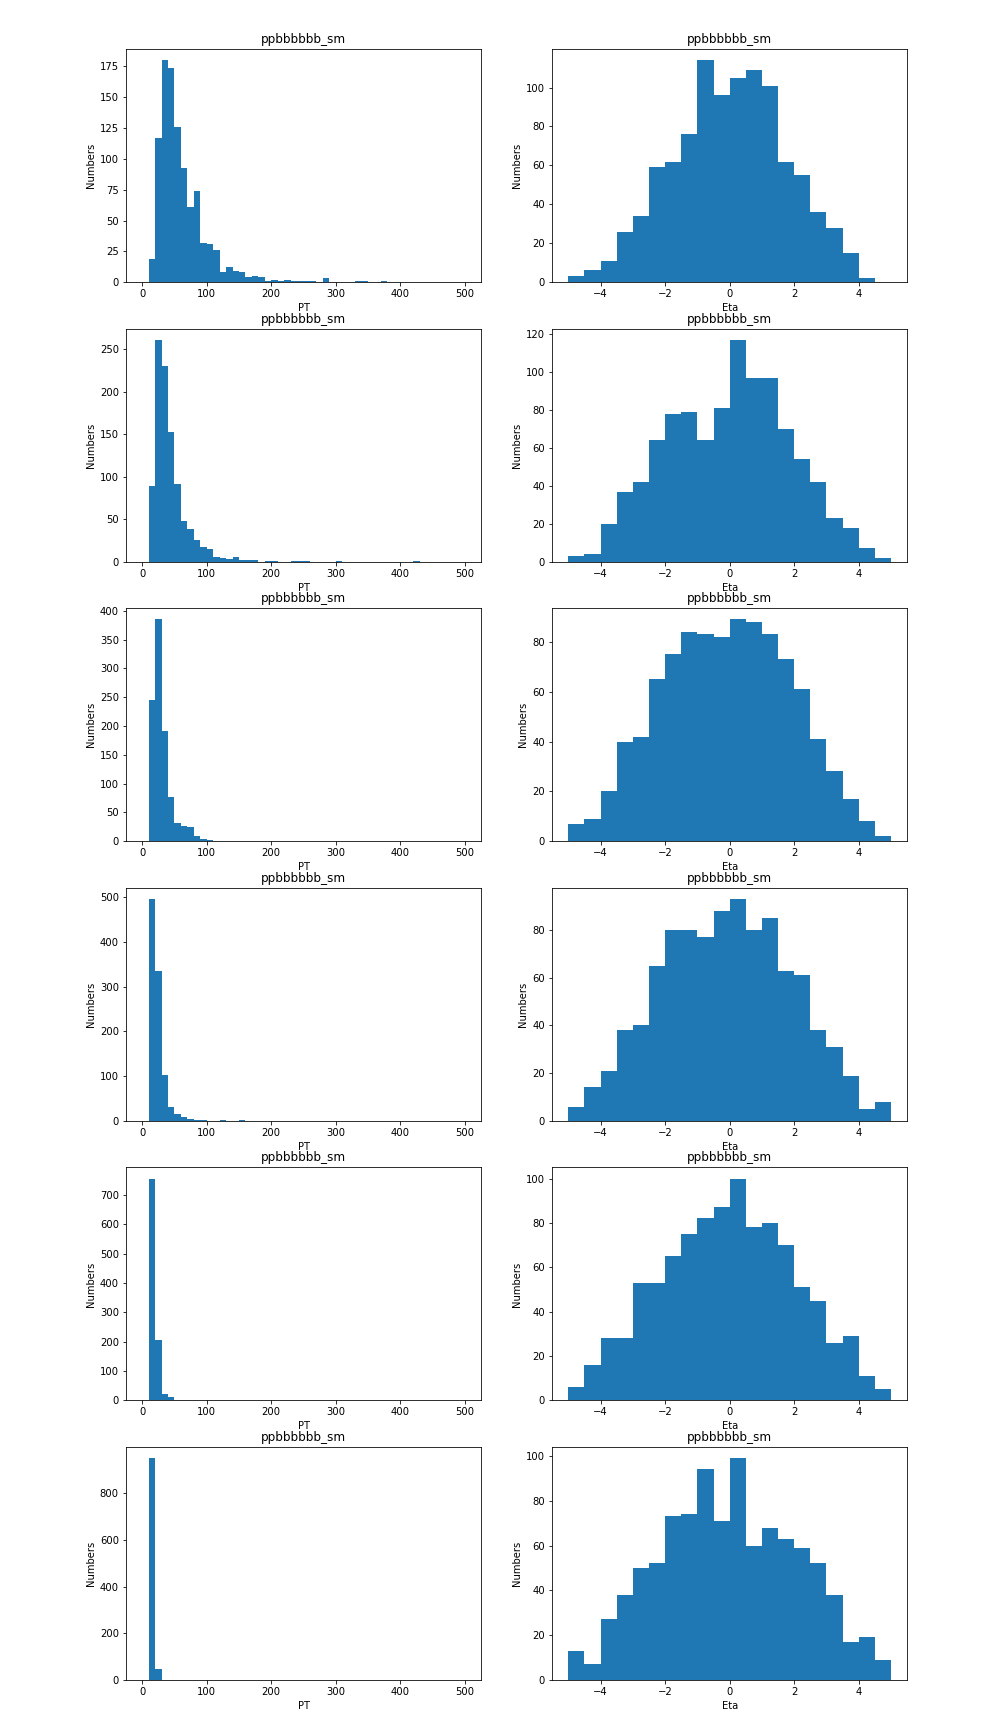
\includegraphics[width=0.8\textwidth]{ppbbbbbb_sm_PT_Eta_order_by_PT.png}
		\caption{$p_\text{T}$ and $\eta$ distributions of b partons for background events. They are ordered by $p_\text{T}$.}
		\label{fig:background_pt_eta_distribution_in_parton_level}
	\end{figure}

	Figure \ref{fig:signal_pt_eta_distribution_in_parton_level} is the $p_\text{T}$ and $\eta$ distributions of b quarks for signal.

	\begin{figure}[htpb]
		\centering
		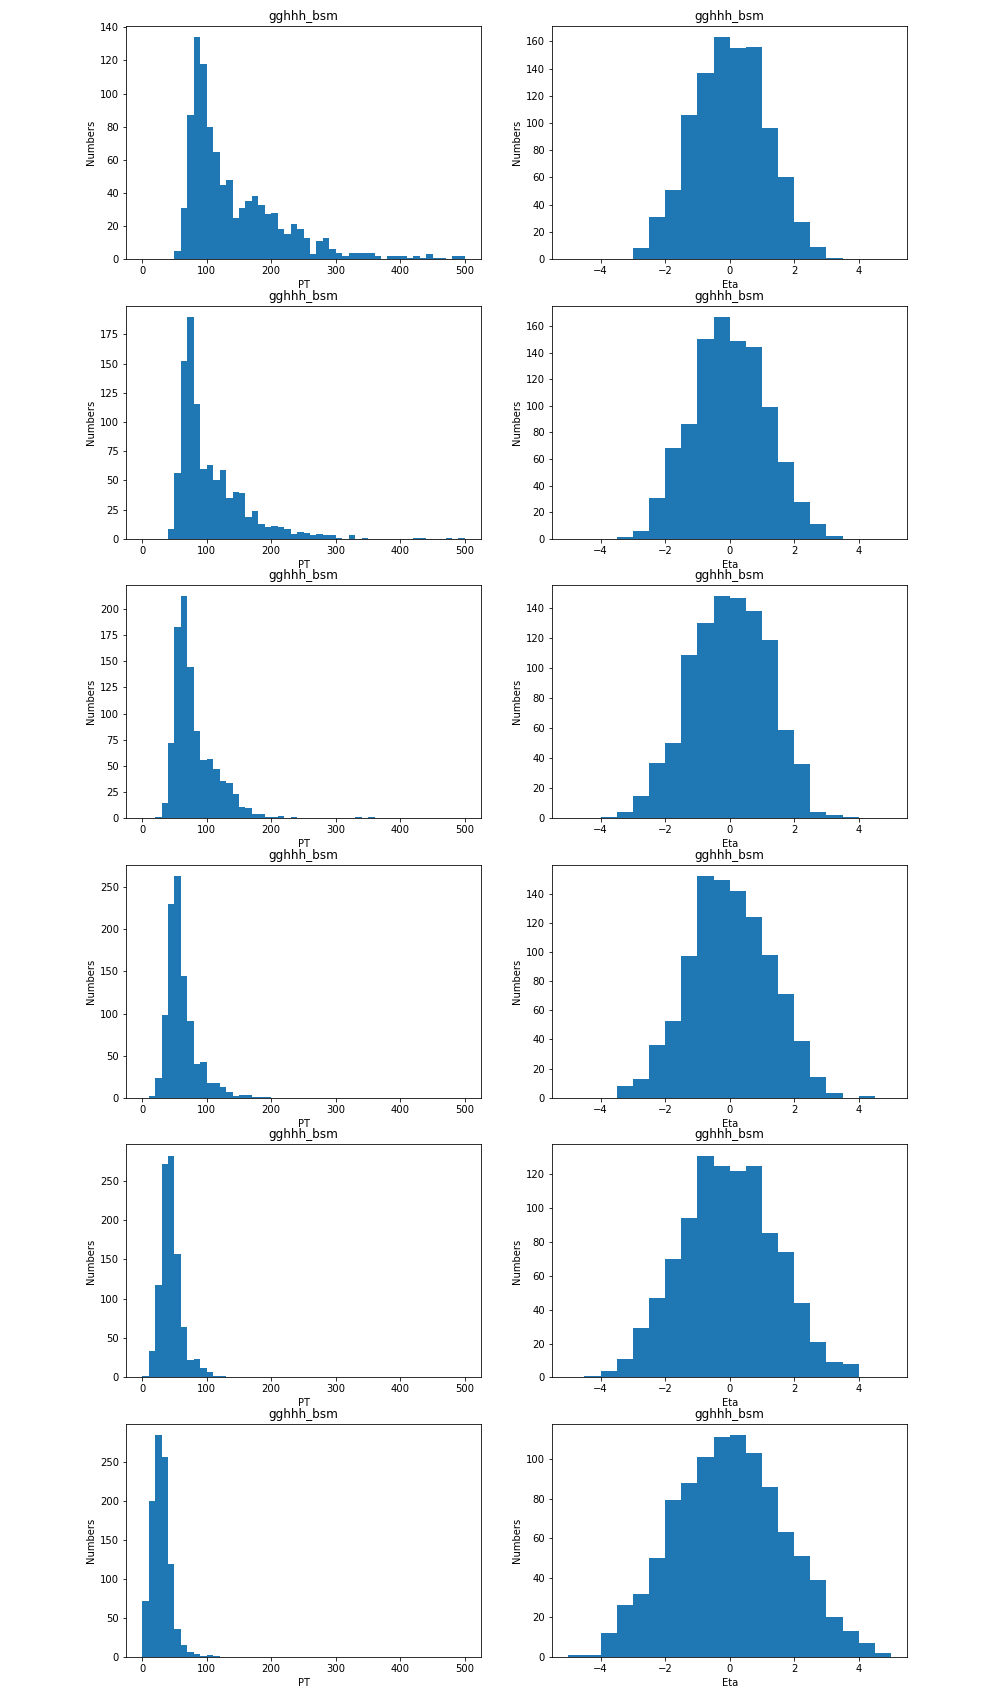
\includegraphics[width=0.8\textwidth]{gghhh_bsm_PT_Eta_order_by_PT.png}
		\caption{$p_\text{T}$ and $\eta$ distributions of b partons for signal events. They are ordered by $p_\text{T}$.}
		\label{fig:signal_pt_eta_distribution_in_parton_level}
	\end{figure}
% section transverse_momentum_and_pseudorapidity_distribution (end)
\section{Delta R and transverse momentum distribution}% (fold)
\label{sec:delta_r_and_transverse_momentum_distribution}
	For signal, I plot the $\Delta R(\text{b,b})$ distribution of two b decays from the same Higgs. Then I plot $\Delta R(\text{b,b})$ against $p_\text{T}(\text{b,b})$. The result is in Figure \ref{fig:dR(b,b)_and_pT(b,b)}. As can be seen from the plot, $\Delta R$ get smaller at higher $p_\text{T}(\text{b,b})$. 
	\begin{figure}[htpb]
		\centering
		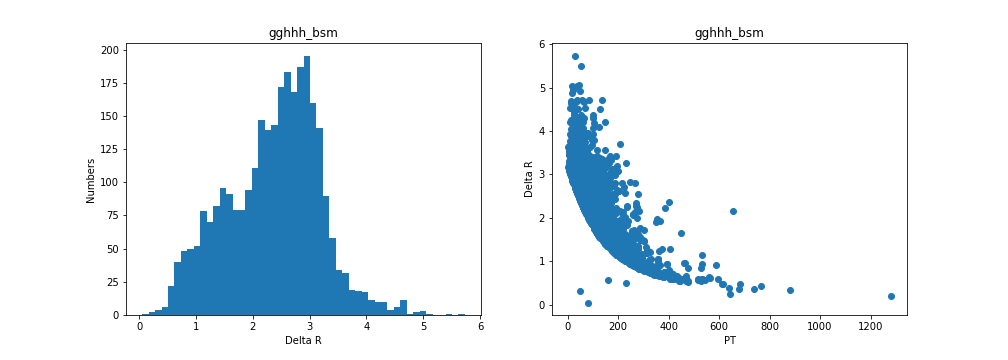
\includegraphics[width=1\textwidth]{gghhh_bsm_bb_Delta_R.png}
		\caption{$\Delta R(\text{b,b})$ distribution and $\Delta R(\text{b,b})$ against $p_\text{T}(\text{b,b})$ plot}
		\label{fig:dR(b,b)_and_pT(b,b)}
	\end{figure}
% section delta_r_and_transverse_momentum_distribution (end)
\section{Cutflow table}% (fold)
\label{sec:cutflow_table}
I apply the $\eta$ and $p_\text{T}$ cuts sequentially and count how many events can pass the cuts. The results are in Table \ref{tab:cutflow_table_background} and Table \ref{tab:cutflow_table_signal}.
	\begin{table}[htpb]
		\centering
		\caption{1000 background events. Those background events is generated in $\sqrt{s} = 13 \text{ TeV}$ with the cut b $p_\text{T} > 10 \text{ GeV}$ in MadGraph.
}
		\label{tab:cutflow_table_background}
		\begin{tabular}{cc}
			Cut & number of events pass \\
			\hline
			6 b-partons $\abs{\eta}<2.5$ & 330 \\
			6 b-partons $p_\text{T} < 25 \text{ GeV}$ & 11 \\
			4 b-partons $p_\text{T} < 40 \text{ GeV}$ & 8                            
		\end{tabular}	
	\end{table}
	
	\begin{table}[htpb]
		\centering
		\caption{1000 signal events.}
		\label{tab:cutflow_table_signal}
		\begin{tabular}{cc}
			Cut & number of events pass \\ 
			\hline
			6 b-partons $\abs{\eta}<2.5$ & 732 \\
			6 b-partons $p_\text{T} < 25 \text{ GeV}$ & 534 \\
			4 b-partons $p_\text{T} < 40 \text{ GeV}$ & 498                            
		\end{tabular}	
	\end{table}
% section cutflow_table (end)

\section{Construction of bb-pairs}% (fold)
\label{sec:construction_of_bb_pairs}
	To construct the bb-pairs from the same Higgs, the typical strategy is to try all combinatoric and find the minimal mass difference between all pairs, i.e. minimize this
	\[
		\chi^2 = [M(\text{b}_1\text{b}_2) - M(\text{b}_3 \text{b}_4)]^2 + [M(\text{b}_1\text{b}_2) - M(\text{b}_5 \text{b}_6)]^2 +[M(\text{b}_3\text{b}_4) - M(\text{b}_5 \text{b}_6)]^2
	\] 
	where $M(\text{b}_i \text{b}_j)$ means the invariant mass of b-parton $i$ and b-parton $j$.

	The other strategy is to minimize mass difference to the SM Higgs mass
	\[
		\chi^2 = [M(\text{b}_1\text{b}_2) - M_\text{H}]^2 + [M(\text{b}_3\text{b}_4) - M_\text{H}]^2 +[M(\text{b}_5\text{b}_6) - M_\text{H}]^2
	\] 

	I implement these two methods to construct bb-pairs and test on the 10,000 signal events at the parton level. The result is as follows:
	\begin{itemize}
		\item Method 1 (mass difference between all pairs): accuracy = 0.863
		\item Method 2 (mass difference to the SM Higgs mass): accuracy = 0.875
	\end{itemize}


	Method 2 is better for identifying the true Higgs pair.
% section construction_of_bb_pairs (end)

\section{Absolute cross section}% (fold)
\label{sec:absolute_cross_section}
	The absolute cross section is defined as follows
	\[
		\sigma_\text{abs} = \sigma \times \frac{\text{number of events pass the cut}}{\text{number of events}}
	\] 

	I have generated background events with different cuts in MadGraph, the detailed information of cuts is in Table \ref{tab:cut_of_different_run}. I calculate their absolute cross section and check if it is the same or not. The result is in Table \ref{tab:absolute_cross_section}.

	\begin{table}[htpb]
		\centering
		\caption{The cuts applied on the different runs. Where $p_\text{T}$ means the minimum transverse momentum of b and $\abs{\eta}$ means the range of b (-1 means no restriction).}
		\label{tab:cut_of_different_run}
		\begin{tabular}{ccc}
			No.& $p_\text{T}$ (GeV) & $\abs{\eta}$  \\
			1 &      0       &           -1      \\
			2 &      10       &     5          \\
			3 &      10       &     3 \\
			4 &      20       &     3 \\
			5 &      0       &     -1 \\
			6 &      10       &     -1 
		\end{tabular}	
	\end{table}


	\begin{table}[htpb]
		\centering
		\caption{Absolute cross section. Where the selection cut is $p_\text{T}> \text{20 GeV}, \abs{\eta} < 3$.}
		\label{tab:absolute_cross_section}
		\begin{tabular}{llllll}
			No.& total event & cross section & events pass selection   & absolute cross section \\
			1& 339 & 2731.9362 & 0 & 0.0    \\
			2& 4761 & 71.316651 & 190 & 2.846   \\
			3& 9054 & 35.225852 & 694 & 2.700 \\
			4& 4207 & 2.7698473 & 4183 & 2.754 \\
			5& 1000 & 2531.9304 & 0 & 0.0 \\
			6& 1000 & 70.158431 & 27 & 1.894
		\end{tabular}	
	\end{table}

	From Table \ref{tab:absolute_cross_section}, if the number of events is large enough the absolute cross section will be similar.
% section absolute_cross_section (end)
\section{The problem for generating \texorpdfstring{pp $\to$ 6b}{pp to 6b} events}% (fold)
\label{sec:the_problem_for_generating_pp_6b_events}
	\href{https://answers.launchpad.net/mg5amcnlo/+question/701314}{Failed to generate the requested number of events}
% section the_problem_for_generating_pp_6b_events (end)	
\section{\texorpdfstring{pp $\to $ 4b}{pp to 4b}}% (fold)
\label{sec:pp_4b}
	I use MadGraph to generate 4b events by following commands:
	\begin{verbatim}
		generate p p > b b b~ b~ 
	\end{verbatim}
	In MadGraph, I apply the cuts: $p_\text{T}>\text{25 GeV}, \abs{\eta}<2.5$ for b. Pass those events through Pythia, then check how many events there are 6 b-hadrons in the final state.

	In 100,000 events, 6,916 events are having greater than or equal to 6 b-hadrons. The distribution of number of b-hadrons is in Figure \ref{fig:number_of_b_hadron}.
	\begin{figure}[htpb]
		\centering
		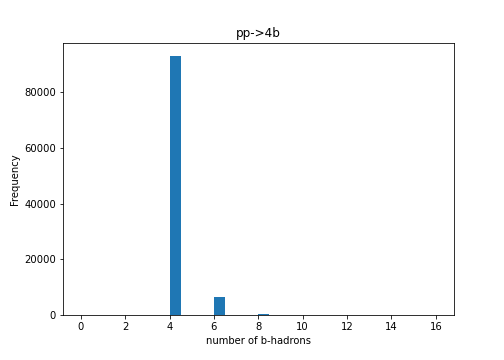
\includegraphics[width=0.8\textwidth]{number_of_b-hadrons.png}
		\caption{Number of b-hadrons in Pythia final state.}
		\label{fig:number_of_b_hadron}
	\end{figure}

	Pass events through Delphes. In Delphes the b-tagging efficiency is set to 1.

	Figure \ref{fig:number_of_jet} is the number of jets and number of b-jets distributions. In 100,000 events, 173 events are having greater than or equal to 6 b-jets.
	\begin{figure}[htpb]
		\centering
		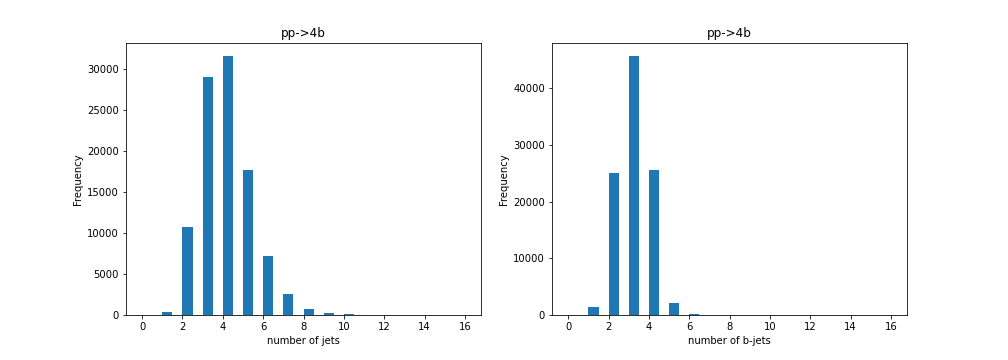
\includegraphics[width=1\textwidth]{number_of_b-jets.png}
		\caption{Number of jets and number of b-jets.}
		\label{fig:number_of_jet}
	\end{figure}
% section pp_4b (end)

\section{Comparison for \texorpdfstring{pp $\to$ 4b}{pp to 4b} and \texorpdfstring{pp $\to$ 6b}{pp to 6b} event}% (fold)
\label{sec:comparison_for_pp_4b_and_pp_6b_event}
	To compare pp->4b and pp->6b events, I plot the $p_\text{T}$, $\eta$ and total invariant mass of 6 b-jets for both.  
	
	The number of events of 6 b-jets for pp->4b is 2051 and for pp->6b is 1408. I scaled the number of events for pp->4b to be the same as pp->6b.

	Figure \ref{fig:pt_eta_distribution_of_b_jets} is $p_\text{T}$ and $\eta$ distributions. Figure \ref{fig:total_invariant_mass_of_b_jets} is total invariant mass of 6 b-jets distributions. Their distributions look similar.

	\begin{figure}[htpb]
		\centering
		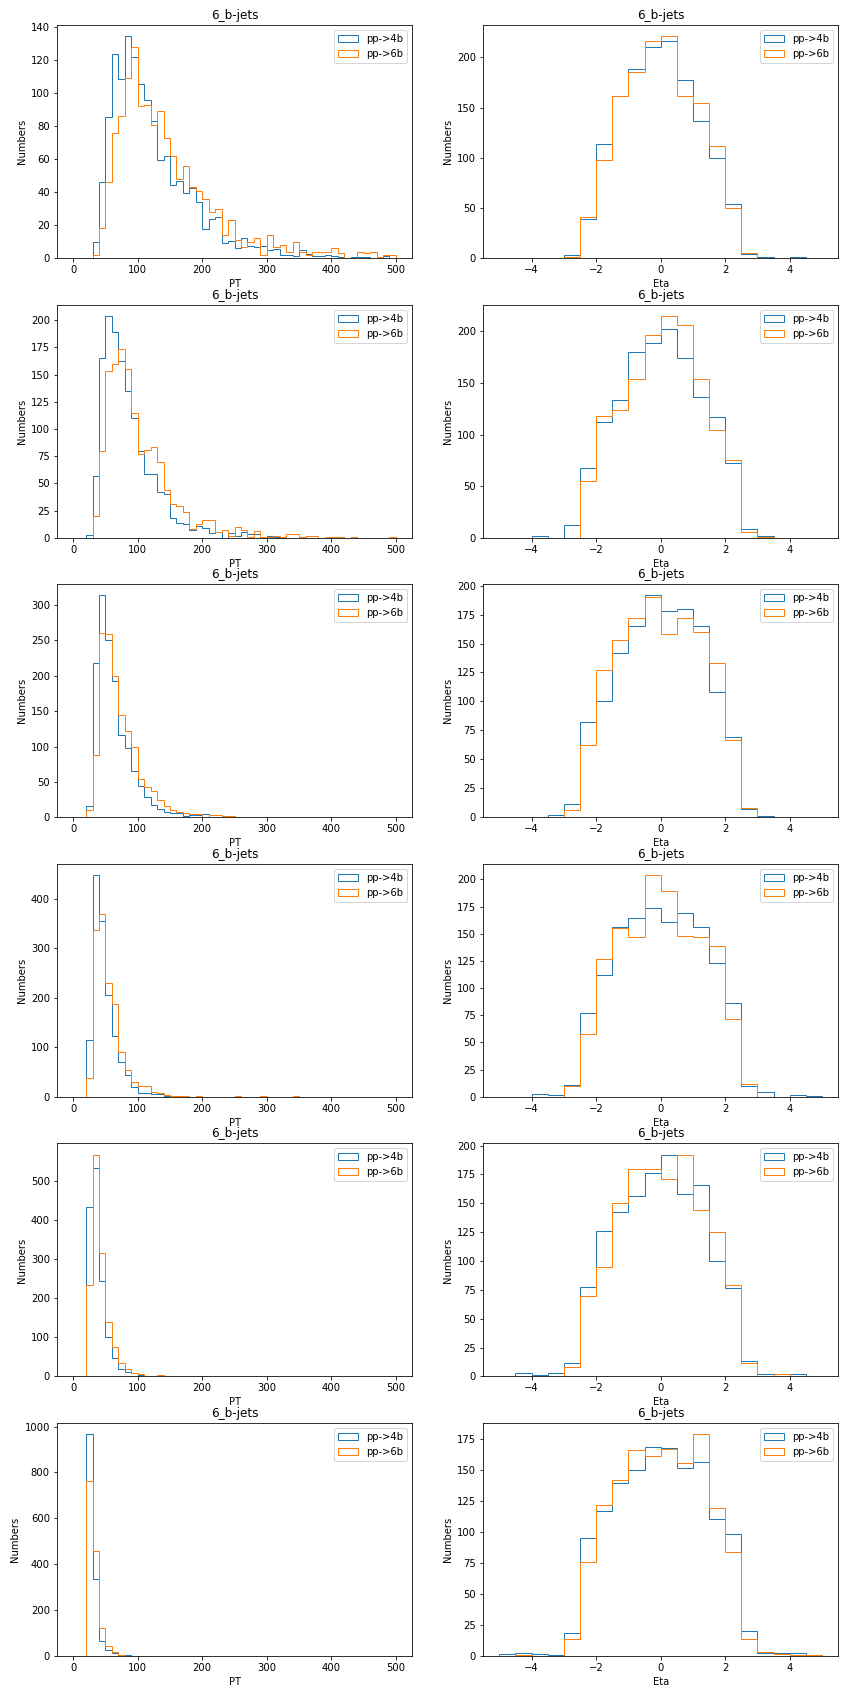
\includegraphics[width=0.7\textwidth]{6_b-jets_PT_Eta_order_by_PT.png}
		\caption{$p_\text{T}$ and $\eta$ distributions of b-jets for pp->4b and pp->6b events. They are ordered by $p_\text{T}$.}
		\label{fig:pt_eta_distribution_of_b_jets}
	\end{figure}
	\begin{figure}[htpb]
		\centering
		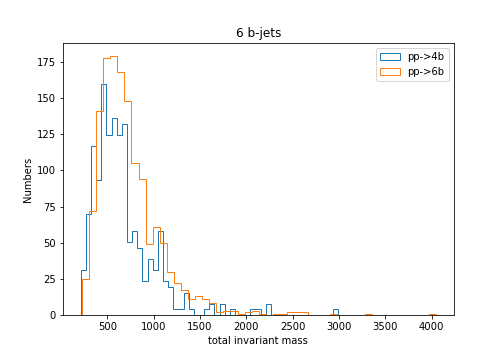
\includegraphics[width=0.7\textwidth]{6_b-jets_total_invariant_mass.png}
		\caption{The distribution of total invariant mass of 6 b-jets for pp->4b and pp->6b events.}
		\label{fig:total_invariant_mass_of_b_jets}
	\end{figure}
	
% section comparison_for_pp_4b_and_pp_6b_event (end)	
\section{Cutflow table for b-jets}% (fold)
\label{sec:cutflow_table_for_b_jets}
	I apply the following cut sequentially and count how many events can pass these cuts. Table \ref{tab:cutflow_table_pp4b_bjet} is the result for pp->4b events. Table \ref{tab:cutflow_table_pp6b_bjet} is the result for pp->6b events. Table \ref{tab:cutflow_table_signal_bjet} is the result for signal events.

	\begin{itemize}
		\item Cut 1: There are greater than or equal to 6 b-jets.
		\item Cut 2: There are greater than or equal to 6 b-jets satisfy $\abs{\eta}<2.5$.
		\item Cut 3: There are greater than or equal to 6 b-jets satisfy $p_\text{T}>\text{25 GeV}$.
		\item Cut 4: There are greater than or equal to 4 b-jets satisfy $p_\text{T}>\text{40 GeV}$.
	\end{itemize}

	\begin{table}[htpb]
		\centering
		\caption{1,000,000 pp->4b events. Those events are generated in $\sqrt{s} = 14 \text{ TeV}$ with the cuts: $p_\text{T} >\text{25 GeV}, \abs{\eta}<2.5$ for b in MadGraph.
}
		\label{tab:cutflow_table_pp4b_bjet}
		\begin{tabular}{cc}
			Cut & number of event pass \\
			\hline
			1 & 1783 \\
			2 & 1565 \\
			3 & 1059 \\
			4 & 735 
		\end{tabular}	
	\end{table}

	\begin{table}[htpb]
		\centering
		\caption{10,000 pp->6b events. Those events are generated in $\sqrt{s} = 14 \text{ TeV}$ with the cuts: $p_\text{T} >\text{25 GeV}, \abs{\eta}<2.5$ for b in MadGraph.
}
		\label{tab:cutflow_table_pp6b_bjet}
		\begin{tabular}{cc}
			Cut & number of event pass \\
			\hline
			1 & 1408 \\
			2 & 1322 \\
			3 & 1052 \\
			4 & 822 
		\end{tabular}	
	\end{table}

	\begin{table}[htpb]
		\centering
		\caption{100,000 signal events. Those events are generated in $\sqrt{s} = 14 \text{ TeV}$.}
		\label{tab:cutflow_table_signal_bjet}
		\begin{tabular}{cc}
			Cut & number of event pass \\
			\hline
			1 & 21,814 \\
			2 & 21,254 \\
			3 & 17,130 \\
			4 & 14,142 
		\end{tabular}	
	\end{table}
% section cutflow_table_for_b_jets (end)

\section{Signal}% (fold)
\label{sec:signal}
	Generate resonant channel gg->h3, h3->h2h, h2->hh in MadGraph by following commands:
	\begin{verbatim}
		import model cxSM_VLF_EFT
		generate g g > h3, (h3 > h2 h, h2 > h h)
	\end{verbatim}
	then check whether this channel is dominated in signal (gg->3h) or not.

	I generate this channel and signal in $\sqrt{s} = \text{14 TeV}$, the cross sections are 2.094 pb and 4.067 pb, respectively.

	Figure \ref{fig:signal_invariant_mass_of_6bjet} is the total invariant mass of 6 b-jets for signal events. Figure \ref{fig:resonant_channel_invariant_mass_of_6bjet} is the total invariant mass of 6 b-jets for this resonant channel. From the results, there is a peak around $\text{400 GeV}$, because the mass of $h_3$ is $m_3 = \text{420 GeV}$.

	\begin{figure}[htpb]
		\centering
		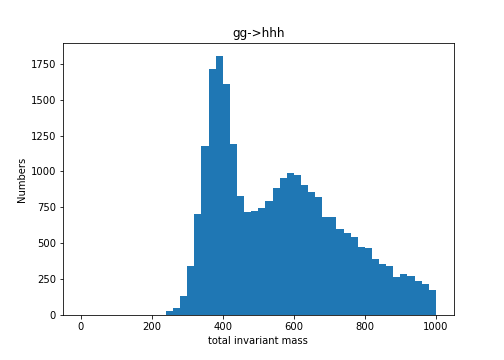
\includegraphics[width=0.8\textwidth]{signal_6_b-jets_total_invariant_mass.png}
		\caption{Total invariant mass of 6 b-jets for signal events.}
		\label{fig:signal_invariant_mass_of_6bjet}
	\end{figure}

	\begin{figure}[htpb]
		\centering
		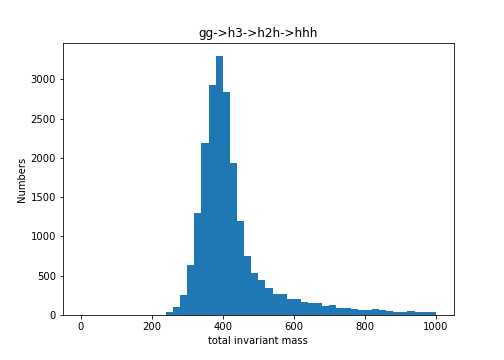
\includegraphics[width=0.8\textwidth]{signal_resonant_6_b-jets_total_invariant_mass.png}
		\caption{Total invariant mass of 6 b-jets for the resonant channel.}
		\label{fig:resonant_channel_invariant_mass_of_6bjet}
	\end{figure}

	A bump around $\text{600 GeV}$ in Figure \ref{fig:signal_invariant_mass_of_6bjet}? In the run card, some parameters are not set correctly. After setting all parameters correctly and regenerating these event, the results are in Figure \ref{fig:invariant_mass_of_6bjet_correct}. There is no bump around $\text{600 GeV}$.

	\begin{figure}[htpb]
		\centering
		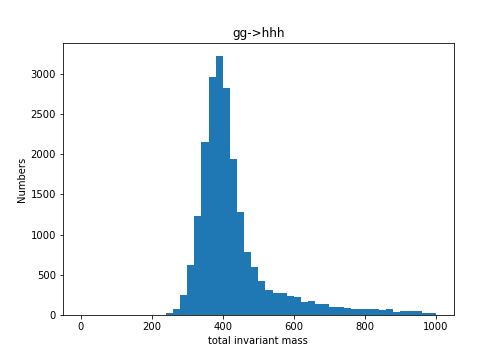
\includegraphics[width=0.49\textwidth]{signal_6_b-jets_total_invariant_mass_correct.png}
		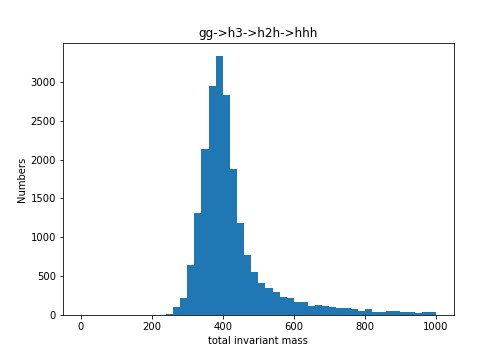
\includegraphics[width=0.49\textwidth]{signal_resonant_6_b-jets_total_invariant_mass_correct.png}
		\caption{Total invariant mass of 6 b-jets for signal events and resonant channel (correct parameters).}
		\label{fig:invariant_mass_of_6bjet_correct}
	\end{figure}



% section signal (end)
	
\section{The cross section in MadGraph}% (fold)
\label{sec:the_cross_section_in_madgraph}
Table \ref{tab:Cross_section_from_MadGraph_and_paper} is the cross sections calculated by MadGraph and in paper. They are different because in MadGraph we only consider LO. But in the paper, the numbers are quoted from the LHC Higgs Cross Section Working Group, and they have considered up to NNLO. The ``k factor'' is around 2.5, which accounts for the values in gg>h3.
	\begin{table}[htpb]
		\centering
		\caption{Cross section from MadGraph and paper}
		\label{tab:Cross_section_from_MadGraph_and_paper}
		\begin{tabular}{ccc}
			Process & $\sigma$  MadGraph (fb)  & $\sigma$ in paper (fb)\\
			\hline
			g g > h3 & 21 & 55 \\
			gg > h3 > h h h & 4.0 &  38.2 \\
			\hline
		\end{tabular}	
	\end{table}

	The problem of cross section: If we use the default run card to generate the decay process, the value of the cross section will be problematic. 

	Solution:
	
	In madevent, use command \verb+compute_widths+ to compute decay widths of $h_2,h_3$, then replace the \verb+run_card.dat+ by \verb+run_card_default.dat+.

	Regenerate the signal and resonant event, the cross sections are $\text{11.1 fb}$ and $\text{10.39 fb}$, respectively. This channel is indeed dominated in the signal.
% section the_cross_section_in_madgraph (end)	
\section{Comparision for \texorpdfstring{pp $\to $ hhh}{pp to hhh} and gg \texorpdfstring{$\to $}{to} hhh}% (fold)
\label{sec:comparision_for_pp_to_hhh_and_gg_to_hhh}
	Generate pp->hhh in MadGraph by following commands:
	\begin{verbatim}
		import model cxSM_VLF_EFT
		define p = p b b~
		generate p p > h h h QCD<=8	
	\end{verbatim}

	Generate gg->hhh in MadGraph by following commands:
	\begin{verbatim}
		import model cxSM_VLF_EFT
		generate g g > h h h	
	\end{verbatim}

	These events are generated in $\text{14 TeV}$ and the sample size is 100k. The cross section for pp->hhh and gg->hhh are $\text{11.22 fb}$ and $\text{11.11 fb}$, respectively. They only differ by 1\%.
% section comparision_for_pp_to_hhh_and_gg_to_hhh (end)		
\section{Comparision for \texorpdfstring{gg $\to $ hhh}{gg to hhh} and resonant channel}% (fold)
\label{sec:comparision_for_gg_hhh_and_resonant_channel}
	To compare $\text{gg $\to $ hhh}$ and resonant channel, I plot the $p_\text{T}$, $\eta$, and total invariant mass of 6 b-jets for both.

	These events are generated in $\text{14 TeV}$ and the sample size is 100k. The cross section for gg->hhh and resonant channel are $\text{11.11 fb}$ and $\text{10.38 fb}$, respectively.

	The number of events of 6 b-jets for gg->hhh is 21,814 and for the resonant channel is 21,475. The numbers are very close. I scaled the number of events for gg->3h to be the same as the resonant channel.

	Figure \ref{fig:signal_resonant_pt_eta_distribution_of_b_jets} is $p_\text{T}$ and $\eta$ distributions. Figure \ref{fig:signal_resonant_total_invariant_mass_of_b_jets} is total invariant mass of 6 b-jets distributions. Their distributions look similar.


	\begin{figure}[htpb]
		\centering
		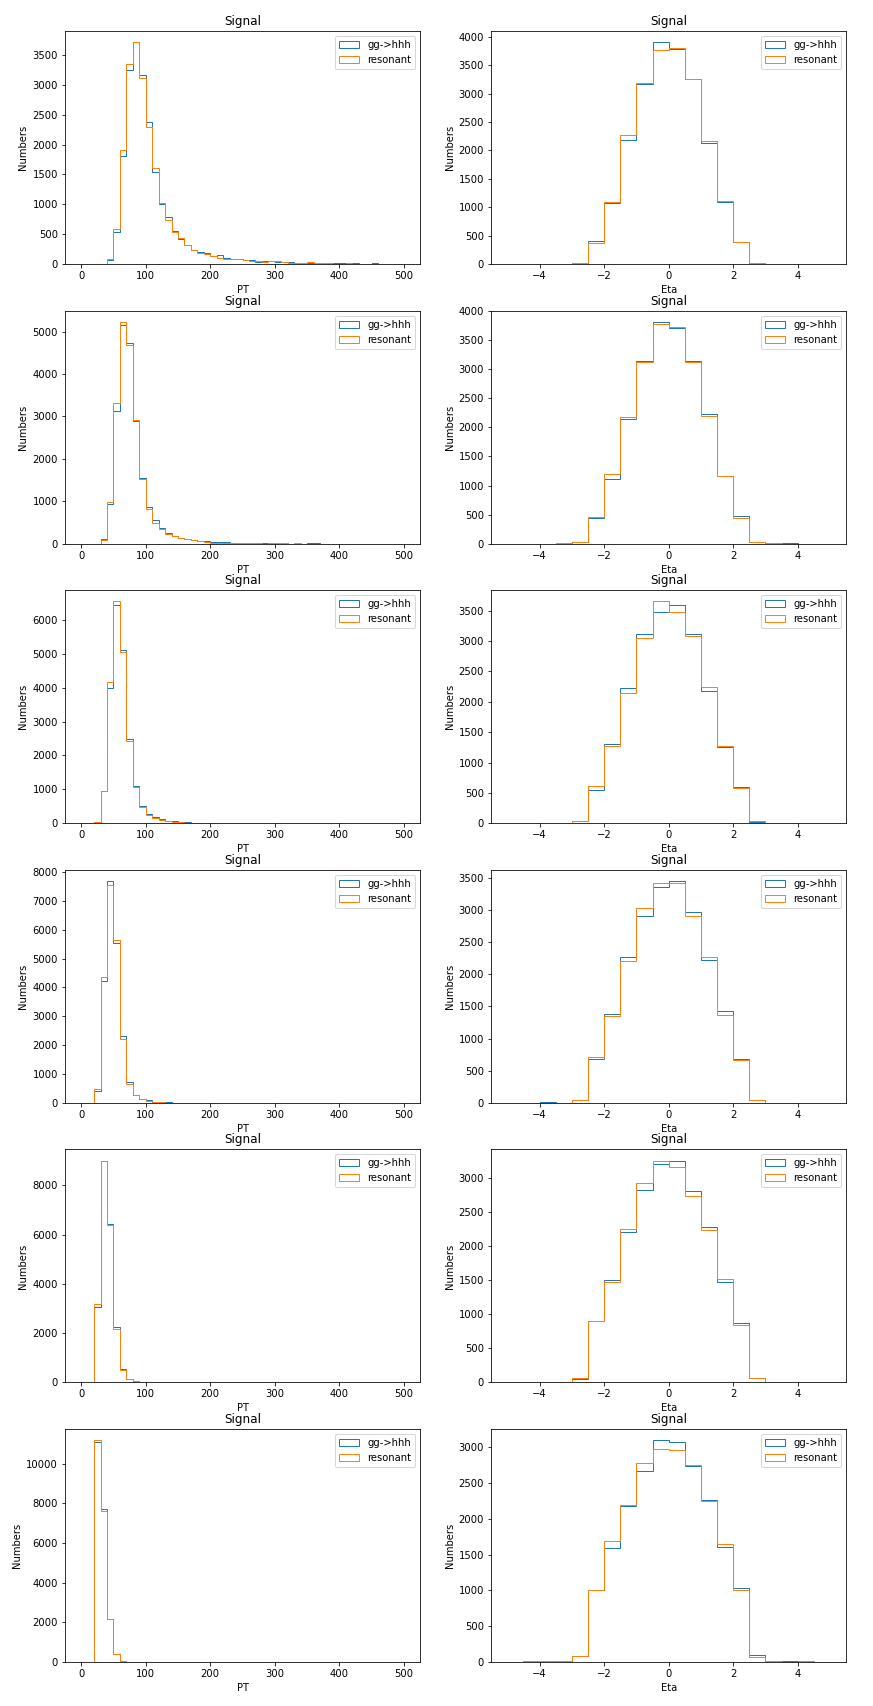
\includegraphics[width=0.7\textwidth]{Signal_PT_Eta_order_by_PT.png}
		\caption{$p_\text{T}$ and $\eta$ distributions of b-jets for gg->3h and resonant channel. They are ordered by $p_\text{T}$.}
		\label{fig:signal_resonant_pt_eta_distribution_of_b_jets}
	\end{figure}
	\begin{figure}[htpb]
		\centering
		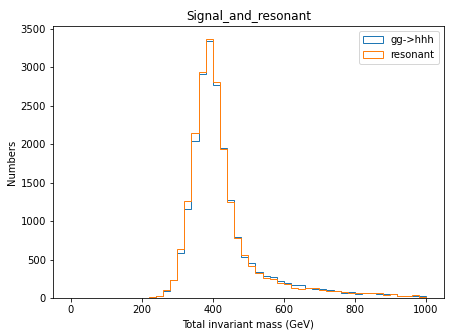
\includegraphics[width=0.7\textwidth]{Signal_and_resonant_total_invariant_mass.png}
		\caption{The distribution of total invariant mass of 6 b-jets for gg->3h and resonant channel.}
		\label{fig:signal_resonant_total_invariant_mass_of_b_jets}
	\end{figure}

	I apply the cuts same in Sec.\ref{sec:cutflow_table_for_b_jets} and count how many events can pass these cuts. Table \ref{tab:cutflow_table_signal_and_resonant_bjet} is the result. The results for both events are similar.
	\begin{table}[htpb]
		\centering
		\caption{Number of events pass the selection cuts. The total number of events for gg->hhh and the resonant channel is 100,000.}
		\label{tab:cutflow_table_signal_and_resonant_bjet}
		\begin{tabular}{ccc}
			Cut &  gg->3h & resonant channel \\
			\hline
			1 & 21,814 & 21,475\\
			2 & 21,254 & 20,898\\
			3 & 17,130 & 16,828\\
			4 & 14,142 & 13,730
		\end{tabular}	
	\end{table}

% section comparision_for_gg_hhh_and_resonant_channel (end)		
\section{Branching ratios and decay widths}% (fold)
\label{sec:branching_ratios_and_decay_widths}
	The branching ratios and decay widths are calculated by MadGraph and Mathematica notebook. Mathematica notebook does not include uu dd ss ee decay modes. Since the contribution of these modes is very small. 

	Table \ref{tab:MG_decay_widths_BR} is calculated by MadGraph. Table \ref{tab:MA_decay_widths_BR} is calculated by Mathematica notebook.
	\begin{table}[htpb]
		\centering
		\caption{Decay widths and branching ratios calculated by MadGraph at BP1.}
		\label{tab:MG_decay_widths_BR}
		\begin{tabular}{lll}
								  & BR        & Width (GeV) \\
			$\text{h}_2\to\text{h}_1\text{h}_1$ & 0.7506    & 0.085616    \\
			$\text{h}_2\to\text{WW}$   & 0.1734    & 0.019782    \\
			$\text{h}_2\to\text{ZZ}$   & 0.07548   & 0.0086097   \\
			$\text{h}_2\to\text{bb}$   & 0.0004724 & 5.3887e-05  \\
			$\text{h}_2\to\text{cc}$   & 3.455e-05 & 3.9407e-06  \\
			$\text{h}_2\to\tau\tau$   & 2.254e-05 & 2.5714e-06  \\
			$\text{h}_2\to\text{ss}$   & 2.185e-07 & 2.4927e-08  \\
			$\text{h}_2\to\text{gg}$   & 1.561e-07 & 1.7811e-08  \\
			$\text{h}_2\to\mu\mu$   & 7.972e-08 & 9.0933e-09  \\
			$\text{h}_2\to\gamma\gamma$   & 6.495e-09 & 7.409e-10   \\
			$\text{h}_2\to\gamma\text{Z}$   & 9.447e-10 & 1.0776e-10  \\
			$\text{h}_2\to\text{dd}$   & 5.441e-10 & 6.207e-11   \\
			$\text{h}_2\to\text{uu}$   & 1.393e-10 & 1.5889e-11  \\
			$\text{h}_2\to\text{ee}$   & 1.865e-12 & 2.1269e-13  \\
			\\
			\\
		\end{tabular}	
		\begin{tabular}{lll}
								  & BR        & Width (GeV) \\
			$\text{h}_3\to\text{h}_1\text{h}_2$ & 0.6795    & 0.8414      \\
			$\text{h}_3\to\text{h}_1\text{h}_1$ & 0.1711    & 0.21183     \\
			$\text{h}_3\to\text{WW}$   & 0.08756   & 0.10842     \\
			$\text{h}_3\to\text{ZZ}$   & 0.04102   & 0.050792    \\
			$\text{h}_3\to\text{tt}$   & 0.02065   & 0.025569    \\
			$\text{h}_3\to\text{gg}$   & 8.662e-05 & 0.00010725  \\
			$\text{h}_3\to\text{bb}$   & 8.158e-05 & 0.00010102  \\
			$\text{h}_3\to\text{cc}$   & 5.961e-06 & 7.3813e-06  \\
			$\text{h}_3\to\tau\tau$   & 3.89e-06  & 4.8167e-06  \\
			$\text{h}_3\to\gamma\gamma$   & 3.852e-07 & 4.7697e-07  \\
			$\text{h}_3\to\gamma\text{Z}$   & 4.937e-08 & 6.1131e-08  \\
			$\text{h}_3\to\text{ss}$   & 3.77e-08  & 4.6686e-08  \\
			$\text{h}_3\to\mu\mu$   & 1.375e-08 & 1.7031e-08  \\
			$\text{h}_3\to\text{dd}$   & 9.389e-11 & 1.1625e-10  \\
			$\text{h}_3\to\text{uu}$   & 2.403e-11 & 2.976e-11   \\
			$\text{h}_3\to\text{ee}$   & 3.217e-13 & 3.9835e-13 
		\end{tabular}
	\end{table}
	\begin{table}[htpb]
		\centering
		\caption{Decay widths and branching ratios calculated by Mathematica at BP1.}
		\label{tab:MA_decay_widths_BR}
		\begin{tabular}{lll}
									  & BR        & Width (GeV) \\
			$\text{h}_2\to\text{h}_1\text{h}_1$     & 0.8321    & 0.1407      \\
			$\text{h}_2\to\text{WW}$       & 0.1166    & 0.019721    \\
			$\text{h}_2\to\text{ZZ}$       & 0.05108   & 0.0086386   \\
			$\text{h}_2\to\text{gg}$       & 0.0001204 & 2.0359e-05  \\
			$\text{h}_2\to\text{bb}$       & 9.91e-05  & 1.6758e-05  \\
			$\text{h}_2\to\tau\tau$       & 1.526e-05 & 2.5802e-06  \\
			$\text{h}_2\to\text{cc}$       & 4.59e-06  & 7.7613e-07  \\
			$\text{h}_2\to\gamma\gamma$       & 3.161e-06 & 5.346e-07   \\
			$\text{h}_2\to\gamma\text{Z}$       & 4.822e-07 & 8.154e-08   \\
			$\text{h}_2\to\mu\mu$μμ       & 5.43e-08  & 9.1826e-09  \\
			$\text{h}_2\to\text{tt}$       & 4.355e-19 & 7.3649e-20  \\
			\\
		\end{tabular}		
		\begin{tabular}{lll}
								  & BR        & Width (GeV) \\
			$\text{h}_3\to\text{h}_1\text{h}_2$ & 0.8219    & 2.158       \\
			$\text{h}_3\to\text{h}_1\text{h}_1$ & 0.1049    & 0.27543     \\
			$\text{h}_3\to\text{WW}$   & 0.04131   & 0.10846     \\
			$\text{h}_3\to\text{ZZ}$   & 0.01941   & 0.050962    \\
			$\text{h}_3\to\text{tt}$   & 0.01242   & 0.032613    \\
			$\text{h}_3\to\text{gg}$   & 6.364e-05 & 0.00016711  \\
			$\text{h}_3\to\text{bb}$   & 1.195e-05 & 3.1386e-05  \\
			$\text{h}_3\to\tau\tau$   & 1.841e-06 & 4.8326e-06  \\
			$\text{h}_3\to\text{cc}$   & 5.536e-07 & 1.4536e-06  \\
			$\text{h}_3\to\gamma\gamma$   & 1.823e-07 & 4.7857e-07  \\
			$\text{h}_3\to\gamma\text{Z}$   & 2.334e-08 & 6.1277e-08  \\
			$\text{h}_3\to\mu\mu$   & 6.55e-09  & 1.7198e-08  
		\end{tabular}
	\end{table}

	The exact values from both are slightly different because MG can not correctly expand the parameter $\epsilon$ in the model.

	Set the $\epsilon$ to $0.001$ and calculate again. The results are in Table \ref{tab:MG_decay_widths_BR_0001} and Table \ref{tab:MA_decay_widths_BR_0001}.

	\begin{table}[htpb]
		\centering
		\caption{Decay widths and branching ratios calculated by MadGraph at BP1 with $\epsilon=0.001$.}
		\label{tab:MG_decay_widths_BR_0001}
		\begin{tabular}{lll}
								  & BR        & Width (GeV) \\
			$\text{h}_2\to\text{h}_1\text{h}_1$ & 0.8311    & 1.4041e-05  \\
			$\text{h}_2\to\text{WW}$   & 0.1174    & 1.9835e-06  \\
			$\text{h}_2\to\text{ZZ}$   & 0.0511    & 8.6329e-07  \\
			$\text{h}_2\to\text{bb}$   & 0.0003198 & 5.4032e-09  \\
			$\text{h}_2\to\text{cc}$   & 2.339e-05 & 3.9513e-10  \\
			$\text{h}_2\to\tau\tau$   & 1.526e-05 & 2.5783e-10  \\
			$\text{h}_2\to\text{ss}$   & 1.479e-07 & 2.4994e-12  \\
			$\text{h}_2\to\mu\mu$μμ   & 5.397e-08 & 9.1178e-13  \\
			$\text{h}_2\to\text{dd}$   & 3.684e-10 & 6.2237e-15  \\
			$\text{h}_2\to\text{uu}$   & 9.431e-11 & 1.5932e-15  \\
			$\text{h}_2\to\text{gg}$   & 1.056e-11 & 1.7841e-16  \\
			$\text{h}_2\to\text{ee}$   & 1.262e-12 & 2.1326e-17  \\
			$\text{h}_2\to\gamma\gamma$   & 4.393e-13 & 7.4213e-18  \\
			$\text{h}_2\to\gamma\text{Z}$   & 6.389e-14 & 1.0794e-18 \\
			\\
			\\
		\end{tabular}
		\begin{tabular}{lll}
								  & BR        & Width (GeV) \\
			$\text{h}_3\to\text{h}_1\text{h}_2$ & 1.0       & 2.1493      \\
			$\text{h}_3\to\text{h}_1\text{h}_1$ & 1.279e-05 & 2.748e-05   \\
			$\text{h}_3\to\text{WW}$   & 5.058e-06 & 1.0871e-05  \\
			$\text{h}_3\to\text{ZZ}$   & 2.369e-06 & 5.0929e-06  \\
			$\text{h}_3\to\text{tt}$   & 1.193e-06 & 2.5638e-06  \\
			$\text{h}_3\to\text{gg}$   & 5.007e-09 & 1.0761e-08  \\
			$\text{h}_3\to\text{bb}$   & 4.713e-09 & 1.0129e-08  \\
			$\text{h}_3\to\text{cc}$   & 3.443e-10 & 7.4011e-10  \\
			$\text{h}_3\to\tau\tau$   & 2.247e-10 & 4.8297e-10  \\
			$\text{h}_3\to\gamma\gamma$   & 2.227e-11 & 4.7857e-11  \\
			$\text{h}_3\to\gamma\text{Z}$   & 2.854e-12 & 6.1335e-12  \\
			$\text{h}_3\to\text{ss}$   & 2.178e-12 & 4.6812e-12  \\
			$\text{h}_3\to\mu\mu$μμ   & 7.945e-13 & 1.7077e-12  \\
			$\text{h}_3\to\text{dd}$   & 5.423e-15 & 1.1657e-14  \\
			$\text{h}_3\to\text{uu}$   & 1.388e-15 & 2.984e-15   \\
			$\text{h}_3\to\text{ee}$   & 1.858e-17 & 3.9942e-17 
		\end{tabular}	
	\end{table}

	\begin{table}[htpb]
		\centering
		\caption{Decay widths and branching ratios calculated by Mathematica at BP1 with $\epsilon=0.001$.}
		\label{tab:MA_decay_widths_BR_0001}
		\begin{tabular}{lll}
								  & BR        & Width (GeV) \\
			$\text{h}_2\to\text{h}_1\text{h}_1$ & 0.8321    & 1.407e-05   \\
			$\text{h}_2\to\text{WW}$   & 0.1166    & 1.9721e-06  \\
			$\text{h}_2\to\text{ZZ}$   & 0.05108   & 8.6386e-07  \\
			$\text{h}_2\to\text{gg}$   & 0.0001204 & 2.0359e-09  \\
			$\text{h}_2\to\text{bb}$   & 9.91e-05  & 1.6758e-09  \\
			$\text{h}_2\to\tau\tau$   & 1.526e-05 & 2.5802e-10  \\
			$\text{h}_2\to\text{cc}$   & 4.59e-06  & 7.7613e-11  \\
			$\text{h}_2\to\gamma\gamma$   & 3.161e-06 & 5.346e-11   \\
			$\text{h}_2\to\gamma\text{Z}$  & 4.822e-07 & 8.154e-12   \\
			$\text{h}_2\to\mu\mu$   & 5.43e-08  & 9.1826e-13  \\
			$\text{h}_2\to\text{tt}$   & 4.355e-15 & 7.3649e-20  \\
			\\
		\end{tabular}
		\begin{tabular}{lll}
								  & BR        & Width (GeV) \\
			$\text{h}_3\to\text{h}_1\text{h}_2$ & 1.0       & 2.158       \\
			$\text{h}_3\to\text{h}_1\text{h}_1$ & 1.276e-05 & 2.7543e-05  \\
			$\text{h}_3\to\text{WW}$   & 5.026e-06 & 1.0846e-05  \\
			$\text{h}_3\to\text{ZZ}$   & 2.361e-06 & 5.0962e-06  \\
			$\text{h}_3\to\text{tt}$   & 1.511e-06 & 3.2613e-06  \\
			$\text{h}_3\to\text{gg}$   & 7.743e-09 & 1.6711e-08  \\
			$\text{h}_3\to\text{bb}$   & 1.454e-09 & 3.1386e-09  \\
			$\text{h}_3\to\tau\tau$   & 2.239e-10 & 4.8326e-10  \\
			$\text{h}_3\to\text{cc}$   & 6.736e-11 & 1.4536e-10  \\
			$\text{h}_3\to\gamma\gamma$   & 2.218e-11 & 4.7857e-11  \\
			$\text{h}_3\to\gamma\text{Z}$   & 2.839e-12 & 6.1277e-12  \\
			$\text{h}_3\to\mu\mu$   & 7.969e-13 & 1.7198e-12  
		\end{tabular}
	\end{table}
	This time, the decay widths and branching ratios calculated by MG and Mathematica notebook become close.

	For color channels, still don't look the same. The reason is that in MadGraph only calculates to LO, but the numbers in the Mathematica notebook are calculated to NLO.
% section branching_ratios_and_decay_widths (end)	
\section{SPANet}% (fold)
\label{sec:spanet}
	Code: \href{https://github.com/Alexanders101/SPANet}{Symmetry Preserving Attention Networks}

	Symmetry Preserving Attention NETworks (Spa-Net) is used to do the jet assignment task. The jet assignment task is the identification of the original particle which leads to a reconstructed jet.

	\subsection{Prepare training data}% (fold)
	\label{sub:prepare_training_data}
		\begin{enumerate}
			\item Defining the event topology in \verb+.ini+ file. The structure of the \verb+.ini+ file follows this format:

			\begin{verbatim}
				[SOURCE]
				FEATURE_1 = FEATURE_OPTION
				FEATURE_2 = FEATURE_OPTION
				FEATURE_3 = FEATURE_OPTION
				...

				[EVENT]
				particles = (PARTICLE_1, PARTICLE_2, ...)
				permutations = EVENT_SYMMETRY_GROUP

				[PARTICLE_1]
				jets = (JET_1, JET_2, ...)
				permutations = JET_SYMMETRY_GROUP

				[PARTICLE_2]
				jets = (JET_1, JET_2, ...)
				permutations = JET_SYMMETRY_GROUP

				...
			\end{verbatim}

			\item Create training dataset in HDF5 format.

			\item Write option-file in JSON format.

		\end{enumerate}
	% subsection prepare_training_data (end)
	\subsection{Training}% (fold)
	\label{sub:training}
		Training:
		\begin{verbatim}
			python train.py -of <OPTIONS_FILE> --log_dir <LOG_DIR>  --name <NAME> --gpus 1
		\end{verbatim}
		\verb+<OPTIONS_FILE>+: JSON file with option overloads. \verb+<LOG_DIR>+: output directory. \verb+<NAME>+: subdirectory name

		Evaluation:
		\begin{verbatim}
			python test.py <log_directory> --gpu
		\end{verbatim}
		\verb+<log_directory>+: directory containing the checkpoint and options file.
		\begin{verbatim}
			python test.py <log_directory> -tf <TEST_FILE> --gpu
		\end{verbatim}
		\verb+<TEST_FILE>+ will replace the test file in the option file.

		Prediction:
		\begin{verbatim}
			python predict.py <log_directory> <output name> -tf <TEST_FILE> --gpu
		\end{verbatim}

	% subsection training (end)	
% section spanet (end)	
\section{SPANet for ttbar event}% (fold)
\label{sec:spanet_for_ttbar_event}
	The training and testing datasets from here: \href{http://mlphysics.ics.uci.edu/data/2021_ttbar/}{Link}

	For full ttbar event:
	\begin{itemize}
		\item Training sample:
		\begin{itemize}
			\item Total sample size: 10,009,520
			\item 2t sample size: 2,967,955
		\end{itemize}
		\item Testing sample size: 
			\begin{itemize}
				\item Total sample size: 358,946
				\item 2t sample size: 116,342
			\end{itemize}
	\end{itemize}

	Figure \ref{fig:full_ttbar_result} is the training results for full ttbar events. 
	\begin{figure}[htpb]
		\centering
		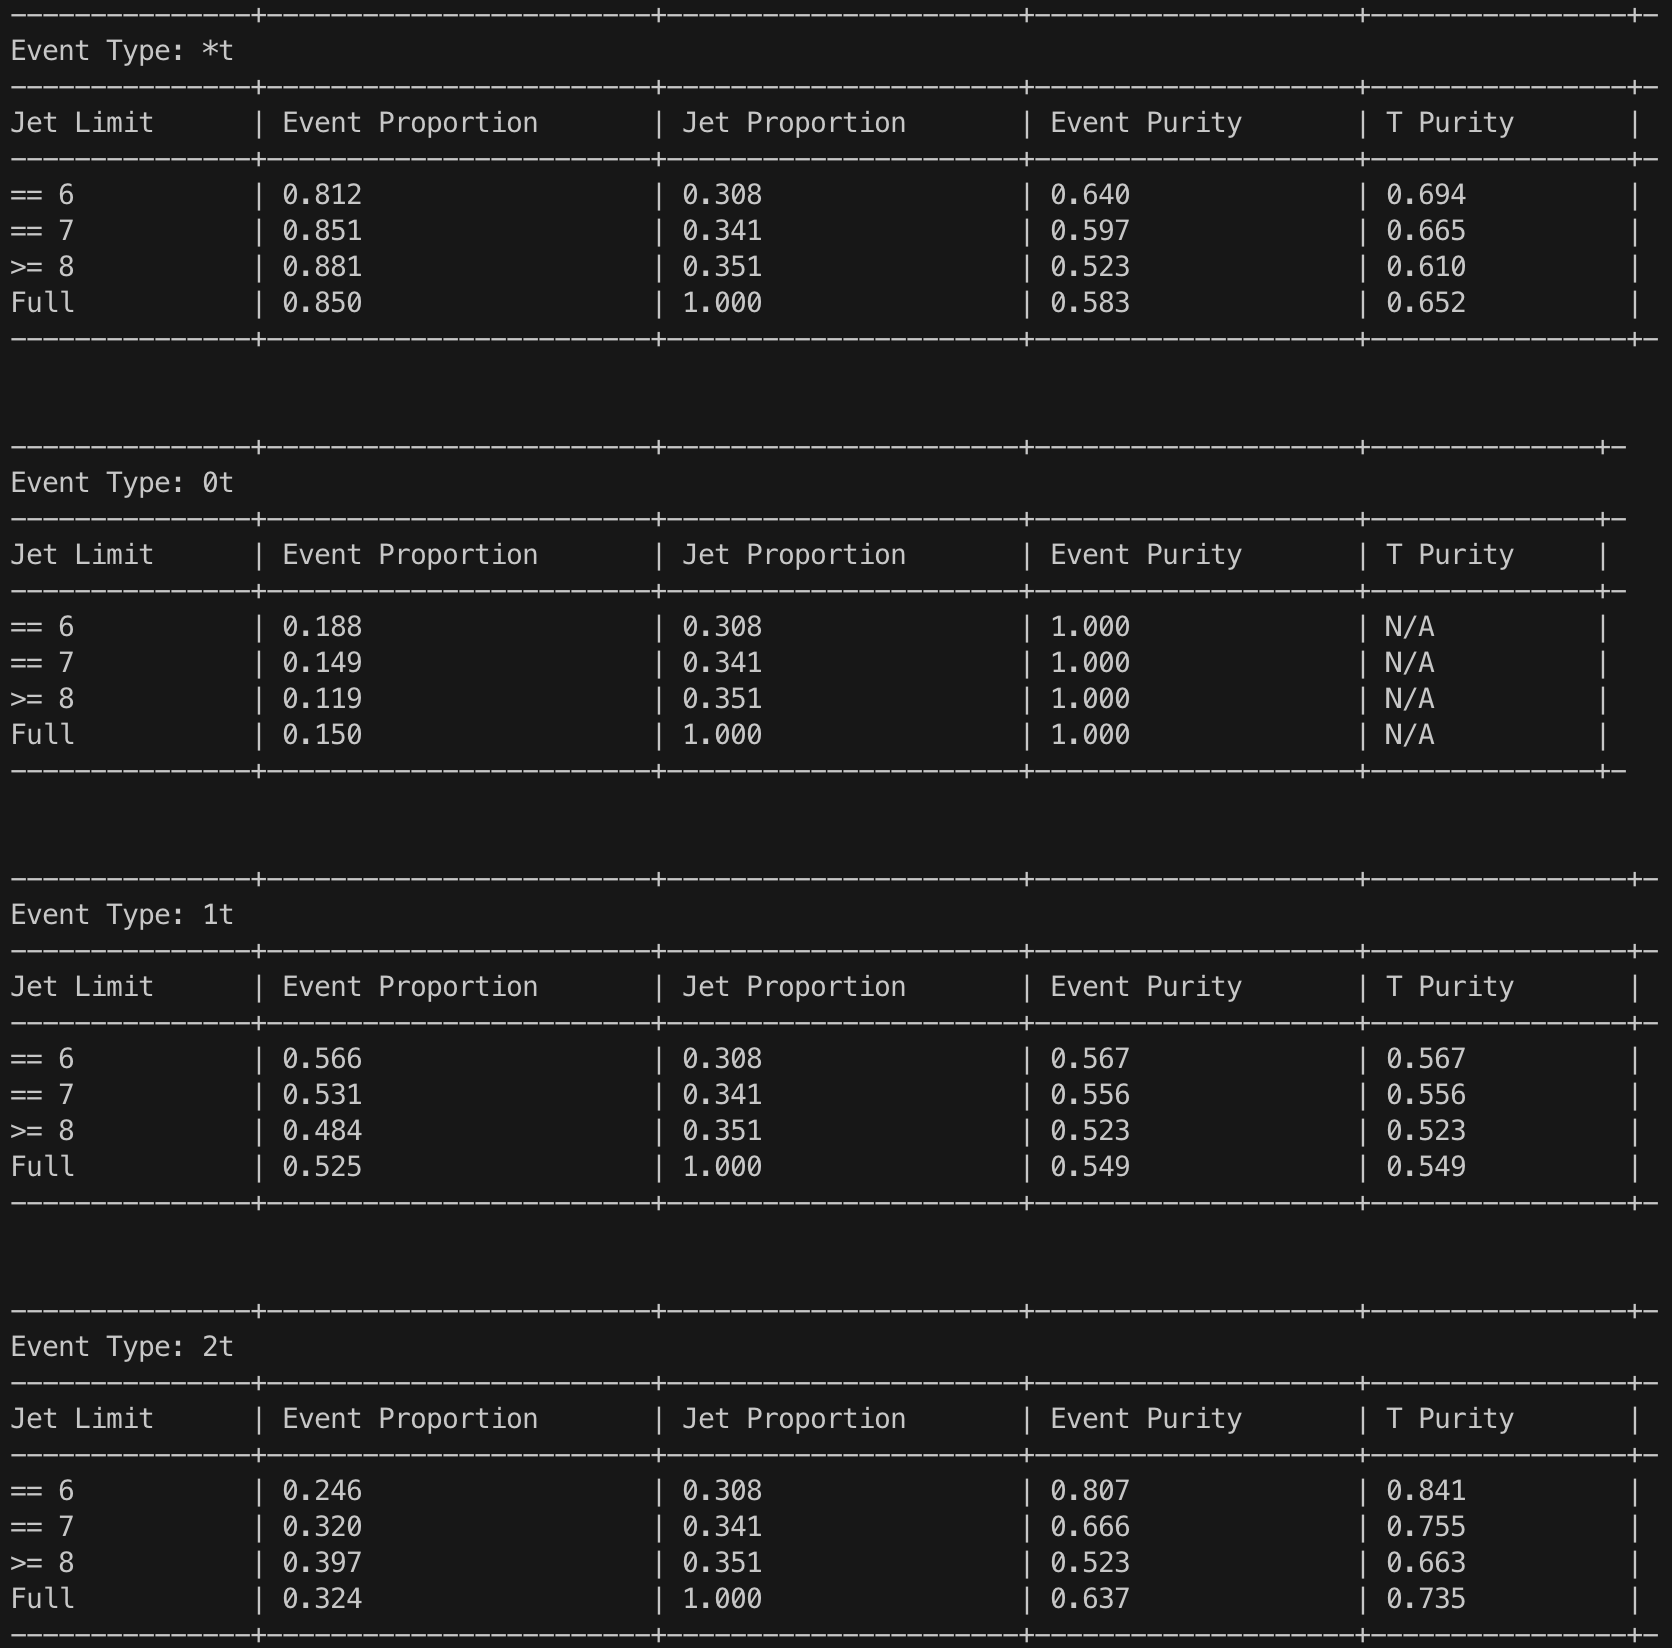
\includegraphics[width=0.8\textwidth]{full_ttbar_training_result.png}
		\caption{The training result for full ttbar events.}
		\label{fig:full_ttbar_result}
	\end{figure}
	The results are the same as the numbers given in the SPANet paper.

% section spanet_for_ttbar_event (end)
\section{SPANet for di-Higgs event}% (fold)
\label{sec:spanet_for_dihiggs_event}
	Generate di-Higgs events in MadGraph by following commands:
	\begin{verbatim}
		import model 2HDMtII_NLO
		generate p p > h2 [QCD] QED<=99 QCD<=99	
	\end{verbatim}
	then use the MadSpin let h2 decay to h1h1 and h1 decay to b$\overline{\text{b}}$. The mass of h2 is $\text{1000 GeV}$.

	The \verb+.ini+ file for di-Higgs event (h > b $\overline{\text{b}}$)
	\begin{verbatim}
		[SOURCE]
		mass = log_normalize
		pt = log_normalize
		eta = normalize
		phi = normalize

		[EVENT]
		particles = (h1, h2)
		permutations = [(h1, h2)]

		[h1]
		jets = (b1, b2)
		permutations = [(b1, b2)]

		[h2]
		jets = (b1, b2)
		permutations = [(b1, b2)]			
	\end{verbatim}

	There are three types of events, 0h, 1h, and 2h. The number means how many identifiable Higgs is in an event.

	Definition of some parameters:
	\begin{itemize}
		\item 	Event proportion:
		\begin{equation}
			\text{Event proportion} \equiv \frac{\text{number of some type events with $i$ jets}}{\text{number of events with $i$ jets}}
		\end{equation}

		\item Jet proportion:
		\begin{equation}
			\text{Jet proportion} \equiv \frac{\text{number of events with $i$ jets}}{\text{total number of events}}
		\end{equation}
		
		\item Event purity:
		\begin{equation}
			\epsilon^{\text{event}} \equiv \frac{\text{number of some type events with and all Higgs are correctly identified}}{\text{number of some type events}} 
		\end{equation}

		\item H purity:
		\begin{equation}
			\epsilon^{\text{h}} \equiv \frac{\text{number of correctly identified Higgs in some type events}}{\text{number of identifiable Higgs in some type events}} 
		\end{equation}
	\end{itemize}

	\subsection{Training sample for di-Higgs events}% (fold)
	\label{sub:training_sample_for_dihiggs_events}
		Di-Higgs events pp->h2, h2->hh, h->bb was generated at $\sqrt{s}= \text{14 TeV}$ using MadGraph. Then pass these events to Pythia8 for showering and hadronization. Then pass to Delphes for detector simulation.
	
		Jets are reconstructed by the anti-kT algorithm with radius $R=0.5$ and are required to have $p_\text{T}\ge \text{20 GeV}$.

		Preselection requirements: $\ge 4$ jets in  $\abs{\eta}<2.5$.

		Define the correct jet assignments by matching them to the simulated truth quarks within an angular distance of $\Delta R = \sqrt{\Delta\eta^2 + \Delta\phi^2}<0.4$.
	% subsection training_sample_for_dihiggs_events (end)

	\subsection{Training result for di-Higgs event}% (fold)
	\label{sub:training_result_for_dihiggs_event}
		For 100k di-Higgs event with $m_{\text{h}_2} = \text{1000 GeV}$:
		\begin{itemize}
			\item Training sample:
			\begin{itemize}
				\item Total sample size: 78,785
				\item 2h sample size: 36,765
				\item 5\% used on validation
			\end{itemize}
			\item Testing sample: 
				\begin{itemize}
					\item Total sample size: 8,753
					\item 2h sample size: 4,130
				\end{itemize}
		\end{itemize}
		\begin{figure}[htpb]
			\centering
			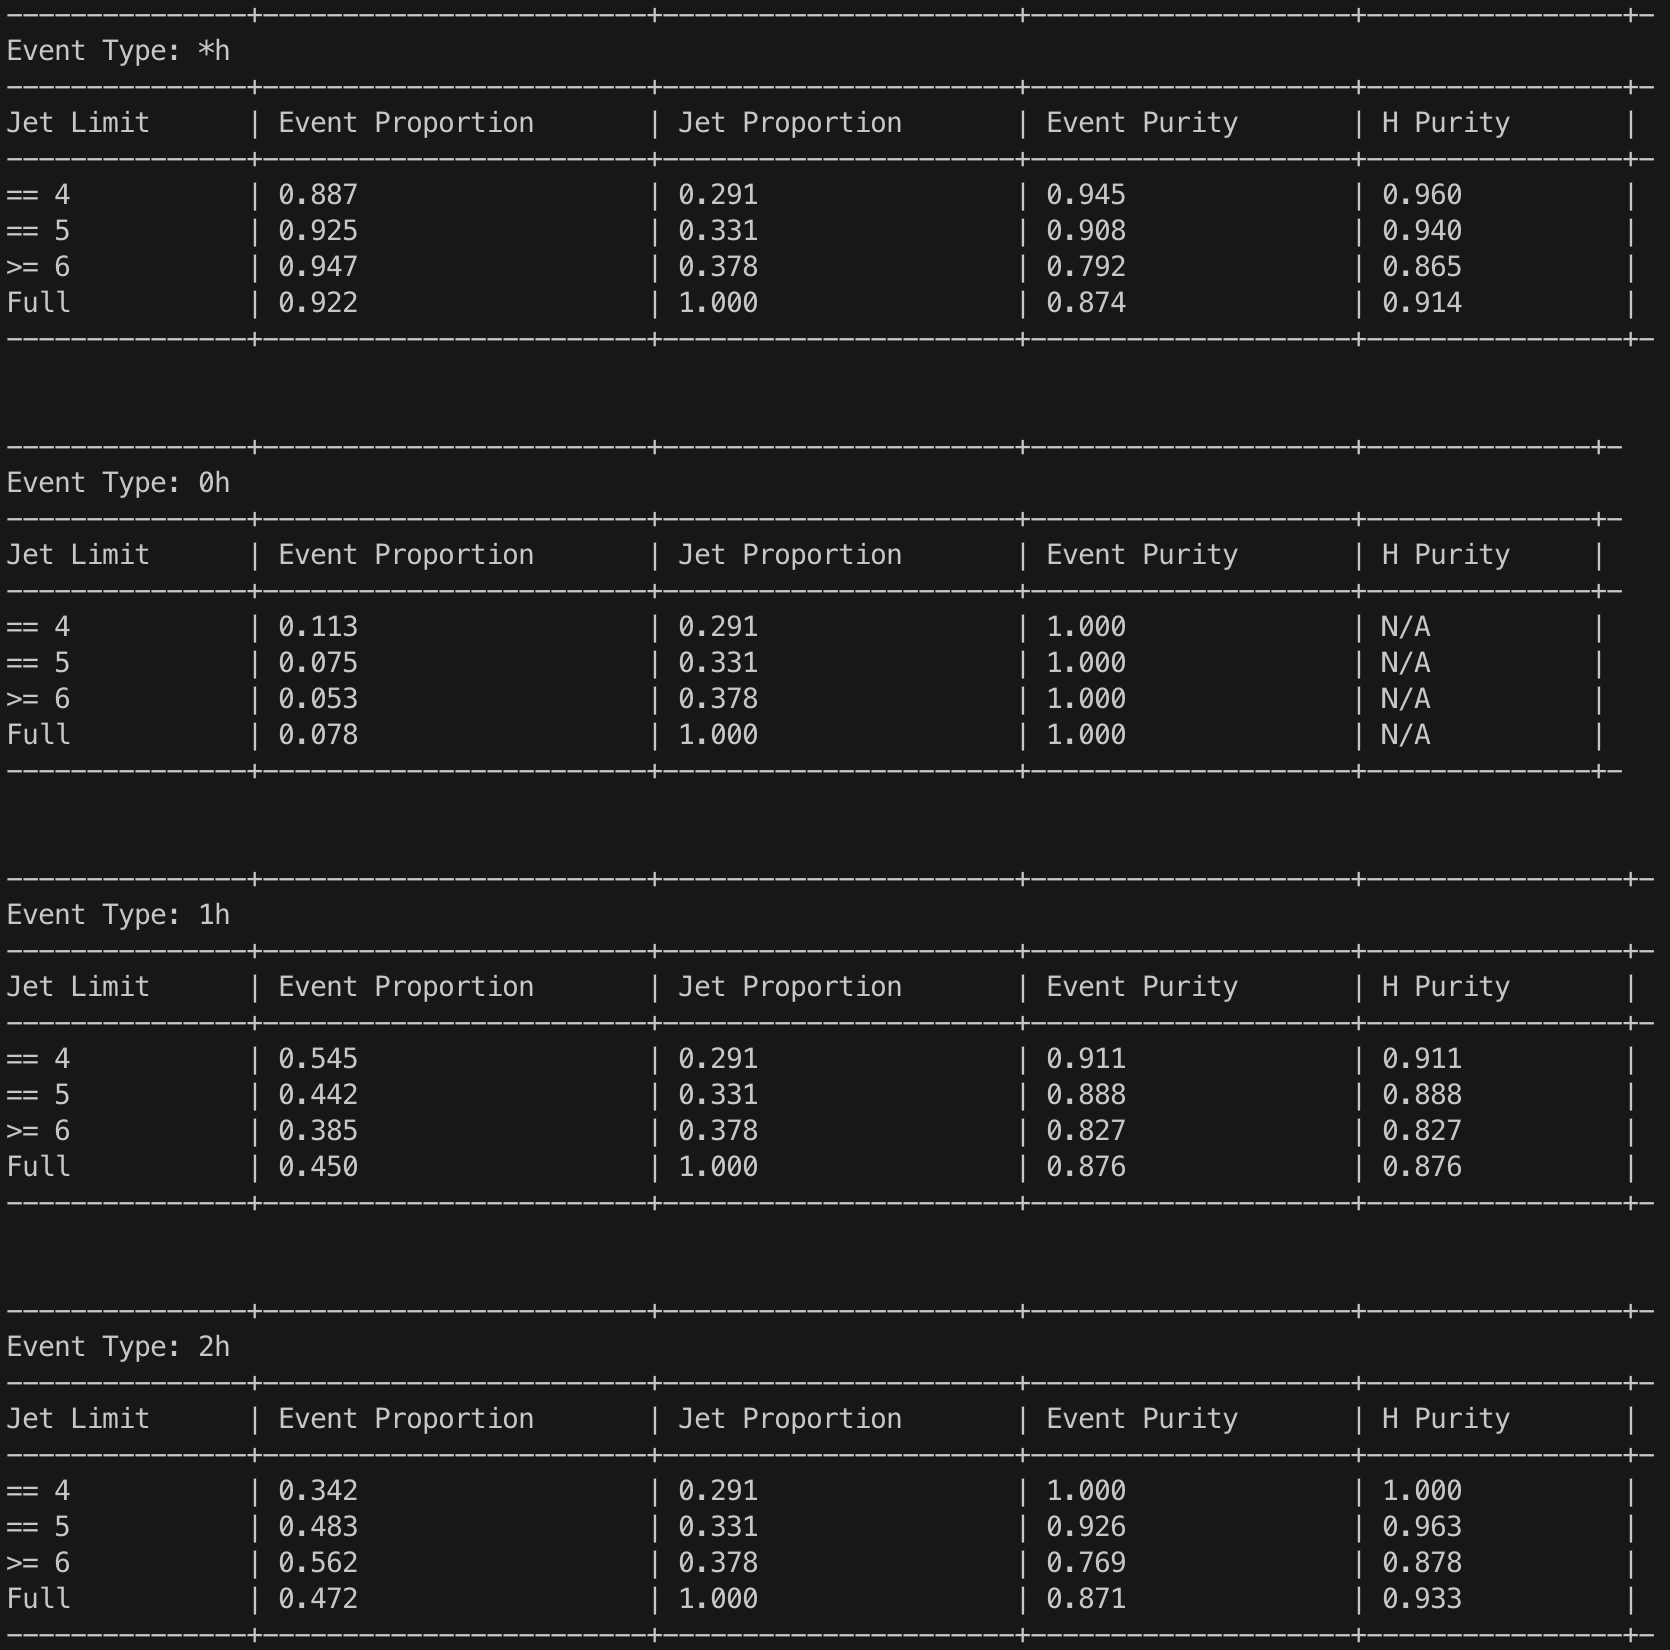
\includegraphics[width=0.8\textwidth]{100k_diHiggs.png}
			\caption{The training result for 100k di-Higgs events.}
			\label{fig:100k_diHiggs_result}
		\end{figure}
		Figure \ref{fig:100k_diHiggs_result} is the training results for 100k di-Higgs events. For 2h events, $\epsilon^{\text{event}} = 0.871, \epsilon^{\text{h}} = 0.933$.

		For 1M di-Higgs event with $m_{\text{h}_2} = \text{1000 GeV}$:
		\begin{itemize}
			\item Training sample:
			\begin{itemize}
				\item Total sample size: 788,160
				\item 2h sample size: 364,773
				\item 5\% used on validation
			\end{itemize}
			\item Testing sample: 
				\begin{itemize}
					\item Total sample size: 87,702
					\item 2h sample size: 40,695
				\end{itemize}
		\end{itemize}
		\begin{figure}[htpb]
			\centering
			\includegraphics[width=0.8\textwidth]{1M_diHiggs.png}
			\caption{The training result for 1M di-Higgs events.}
			\label{fig:1M_diHiggs_result}
		\end{figure}

		Figure \ref{fig:1M_diHiggs_result} is the training results for 1M di-Higgs events. For 2h events, $\epsilon^{\text{event}} = 0.914, \epsilon^{\text{h}} = 0.955$.

		For di-Higgs event with $m_{\text{h}_2} = \text{500 GeV}$:
		\begin{itemize}
			\item Training sample:
			\begin{itemize}
				\item Total sample size: 764,676
				\item 2h sample size: 396,588
				\item 5\% used on validation
			\end{itemize}
			\item Testing sample: 
				\begin{itemize}
					\item Total sample size: 84,687
					\item 2h sample size: 43,818
				\end{itemize}
		\end{itemize}
		\begin{figure}[htpb]
			\centering
			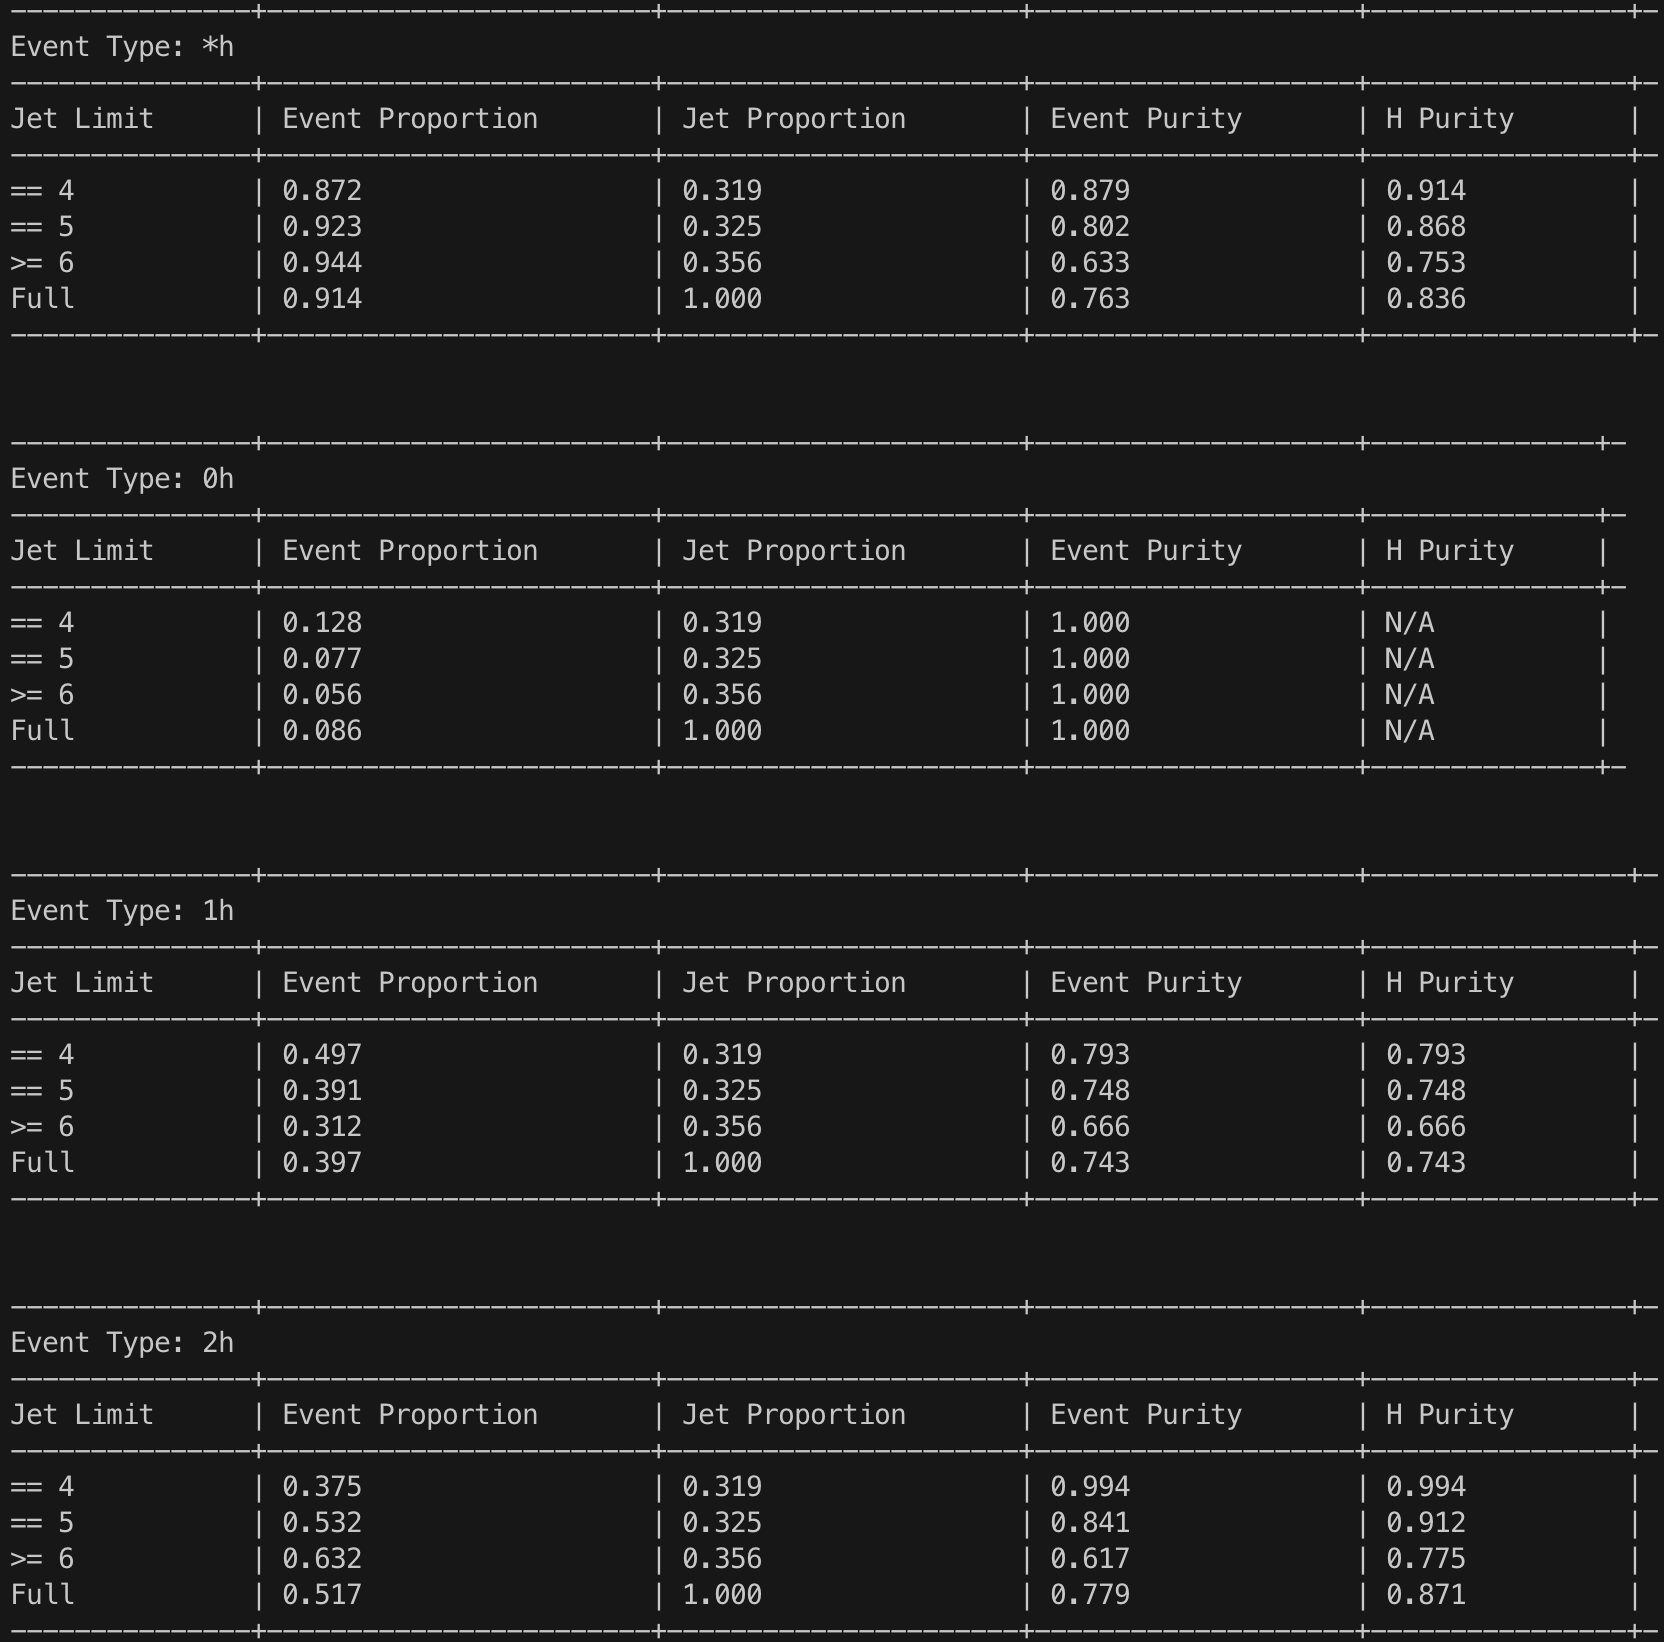
\includegraphics[width=0.8\textwidth]{1M_diHiggs_500_GeV.png}
			\caption{The training result for di-Higgs events with $m_{\text{h}_2} = \text{500 GeV}$.}
			\label{fig:1M_500_GeV_diHiggs_result}
		\end{figure}

		Figure \ref{fig:1M_500_GeV_diHiggs_result} is the training results for $\text{500 GeV}$ di-Higgs events. For 2h events, $\epsilon^{\text{event}} = 0.779, \epsilon^{\text{h}} = 0.871$.

	% subsection training_result_for_dihiggs_event (end)

	\subsection{Apply the pre-trained model on different \texorpdfstring{$m_{\text{h}_2}$}{mh2} sample}% (fold)
	\label{sub:apply_the_pre_trained_model_on_different_mh2_sample}
		The SPANet models in Sec.\ref{sub:training_result_for_dihiggs_event} are trained on $m_{\text{h}_2} = \text{500 GeV}$ and $m_{\text{h}_2} = \text{1000 GeV}$. Test these models on samples with $m_{\text{h}_2} = \text{500 GeV}$, $ \text{750 GeV}$, $\text{1000 GeV}$.

		The results are summarized in Table \ref{tab:SPANet_test_on_different_h2_mass}.
		\begin{table}[htpb]
			\centering
			\caption{SPANet models test on different $m_{\text{h}_2}$ samples.}
			\label{tab:SPANet_test_on_different_h2_mass}
			\begin{tabular}{cccc}
				Training $m_{\text{h}_2}$ (GeV) & Testing $m_{\text{h}_2}$ (GeV) & Event purity & H purity \\
				\hline 
				500      & 500     & 0.779        & 0.871    \\
				500      & 750     & 0.408        & 0.672    \\
				500      & 1000    &  0.390      &  0.665    \\
				1000     & 500    & 0.383        & 0.638   \\
				1000     & 750    & 0.731        & 0.860   \\
				1000     & 1000    & 0.914        & 0.955   
			\end{tabular}
		\end{table}
	% subsection apply_the_pre_trained_model_on_different_mh2_sample (end)

% section spanet_for_dihiggs_event (end)
\section{SPANet for tri-Higgs event}% (fold)
\label{sec:spanet_for_trihiggs_event}
	The tri-Higgs events are signal events (gg->hhh) generated in the previous.

	\subsection{Training sample for tri-Higgs event}% (fold)
	\label{sub:training_sample_for_trihiggs_event}
		Tri-Higgs events gg->hhh was generated at $\sqrt{s} = \text{14 TeV}$ using MadGraph. Then pass these events to Pythia8 for showering and hadronization. In Pythia8, the Higgs is forced to decay to b$\overline{\text{b}}$. Then pass to Delphes for detector simulation.
	
		Jets are reconstructed by the anti-kT algorithm with radius $R=0.5$ and are required to have $p_\text{T}\ge \text{20 GeV}$.

		Preselection requirements: $\ge 6$ jets in  $\abs{\eta}<2.5$.

		Define the correct jet assignments by matching them to the simulated truth quarks within an angular distance of $\Delta R = \sqrt{\Delta\eta^2 + \Delta\phi^2}<0.4$.
	% subsection training_sample_for_dihiggs_event (end)

	\subsection{Training result for tri-Higgs event}% (fold)
	\label{sub:training_result_for_trihiggs_event}
		For 1M tri-Higgs event:
		\begin{itemize}
			\item Training sample:
			\begin{itemize}
				\item Total sample size: 542,681
				\item 3h sample size: 104,467
				\item 5\% used on validation
			\end{itemize}
			\item Testing sample: 
				\begin{itemize}
					\item Total sample size: 60,173
					\item 3h sample size: 11,598
				\end{itemize}
		\end{itemize}
		\begin{figure}[htpb]
			\centering
			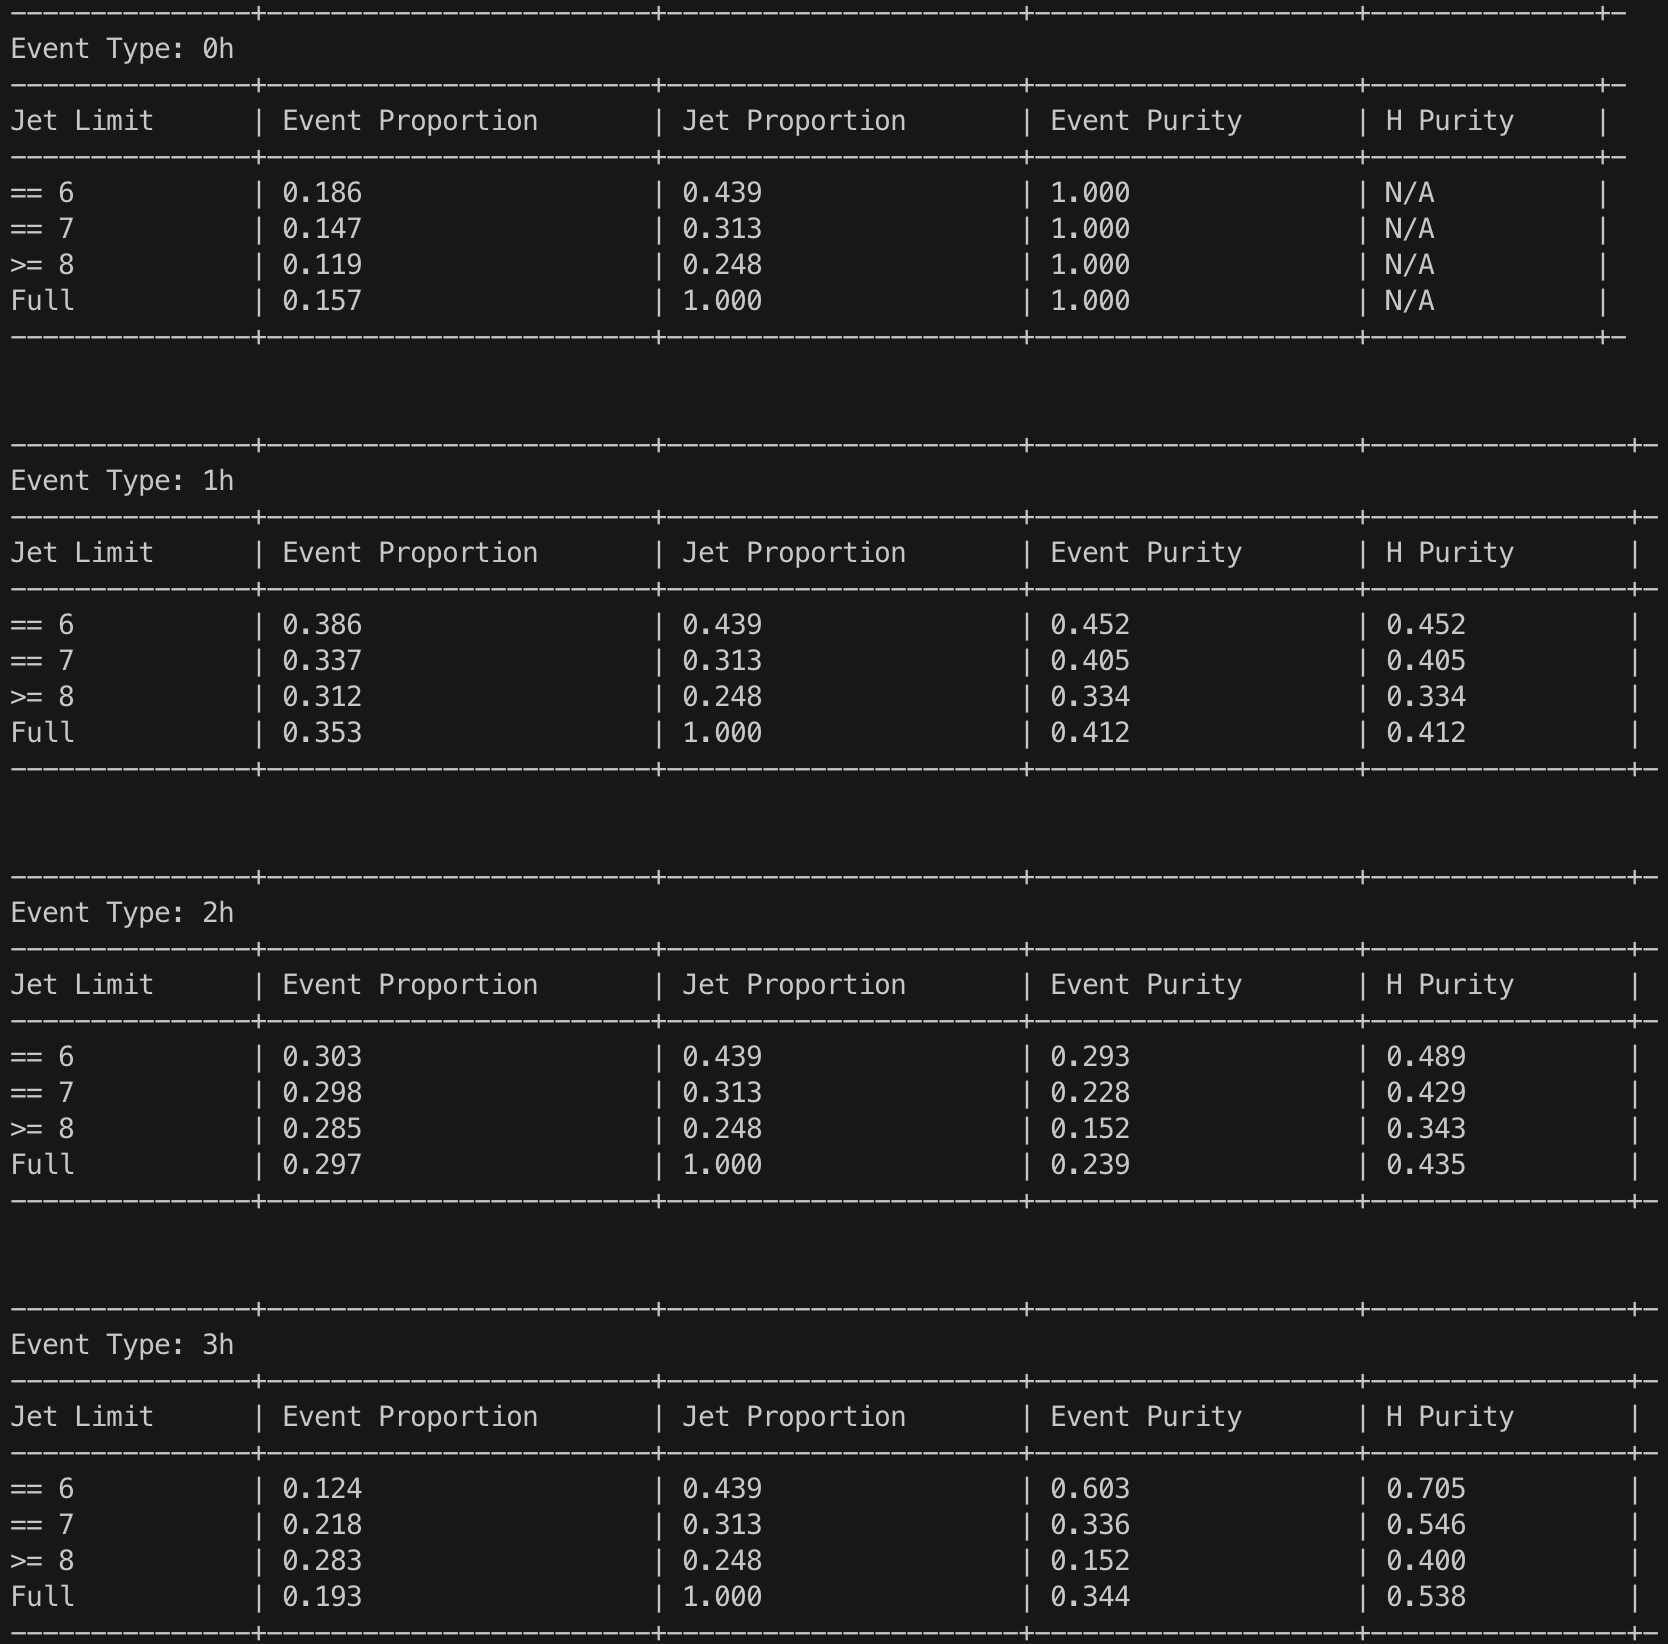
\includegraphics[width=0.8\textwidth]{1M_triHiggs.png}
			\caption{The training result for 1M tri-Higgs events.}
			\label{fig:1M_triHiggs_result}
		\end{figure}

		Figure \ref{fig:1M_triHiggs_result} is the training results for 1M tri-Higgs events. For 3h events, $\epsilon^{\text{event}} = 0.344, \epsilon^{\text{h}} = 0.538$.

	% subsection training_result_for_trihiggs_event (end)	

% section spanet_for_trihiggs_event (end)		

\section{\texorpdfstring{$\chi^2$}{Chi square} method}% (fold)
\label{sec:chi_2_method}
	\subsection{Di-Higgs}% (fold)
	\label{sub:di_higgs}
		Try all possible combinations of final jets and find the minimal mass difference between SM Higgs mass, i.e. minimize this
		\begin{equation}\label{eq:diHiggs_chisq}
			\chi^2 = [M(j_1j_2)-M_\text{H}]^2 + [M(j_3j_4)-M_\text{H}]^2
		\end{equation}
		where $M(j_ij_j)$ means the invariant mass of jet $i$ and jet $j$.

		The results are presented in Table \ref{tab:comparison_SPANet_and_chi2}.

		\begin{table}[htpb]
			\centering
			\caption{Performance comparison for di-Higgs events.}
			\label{tab:comparison_SPANet_and_chi2}
			\begin{tabular}{c|c|cc|cc}
					  & Event    & \multicolumn{2}{|c|}{SPANet Efficiency} & \multicolumn{2}{|c}{ $\chi^2$ Efficiency} \\
				$N_\text{Jet}$ & Fraction & Event             & Higgs             & Event            & Higgs           \\
				\hline
				$=4$	  &   0.224       &     1.000       &   1.000       &   1.000           &    1.000             \\
				$=5$	  &   0.334       &     0.950       &   0.975       &   0.675           &    0.737            \\
				$\ge 6$	  &   0.442       &     0.844       &   0.918		&   0.313           &    0.441            \\
				Total	  &   1.000       &     0.914       &   0.955       &   0.582           &    0.665            
			\end{tabular}
		\end{table}

	% subsection di_higgs (end)
	\subsection{Di-Higgs with b-tag}% (fold)
	\label{sub:di_higgs_with_b_tag}
		Similarly, try to minimize (\ref{eq:diHiggs_chisq}), but only try all possible permutations of b-tagged jets. Here, we only consider the events with $\ge 4$ b-jets.

		The results are presented in Table \ref{tab:comparison_SPANet_and_chi2_diHiggs_with_btag_100} and Table \ref{tab:comparison_SPANet_and_chi2_diHiggs_with_btag_default}.

		\begin{table}[htpb]
			\centering
			\caption{Performance comparison for di-Higgs events with $\ge 4$ b-jets (b-tagging efficiency = 100\%).}
			\label{tab:comparison_SPANet_and_chi2_diHiggs_with_btag_100}
			\begin{tabular}{c|c|cc|cc}
					  & Event    & \multicolumn{2}{|c|}{SPANet Efficiency} & \multicolumn{2}{|c}{ $\chi^2$ Efficiency} \\
				$N_\text{Jet}$ & Fraction & Event             & Higgs             & Event            & Higgs           \\
				\hline
				$=4$	  &   0.224       &     1.000       &   1.000       &   1.000           &    1.000          \\
				$=5$	  &   0.334       &     0.980       &   0.990       &   0.974           &    0.979          \\
				$\ge 6$	  &   0.442       &     0.946       &   0.972		&   0.916           &    0.933          \\
				Total	  &   1.000       &     0.969       &   0.984       &   0.954           &    0.963            
			\end{tabular}
		\end{table}

		\begin{table}[htpb]
			\centering
			\caption{Performance comparison for di-Higgs events with $\ge 4$ b-jets (b-tagging efficiency = default).}
			\label{tab:comparison_SPANet_and_chi2_diHiggs_with_btag_default}
			\begin{tabular}{c|c|cc|cc}
					  & Event    & \multicolumn{2}{|c|}{SPANet Efficiency} & \multicolumn{2}{|c}{ $\chi^2$ Efficiency} \\
				$N_\text{Jet}$ & Fraction & Event             & Higgs             & Event            & Higgs           \\
				\hline
				$=4$	  &   0.200       &     1.000       &   1.000       &   1.000           &    1.000          \\
				$=5$	  &   0.318       &     0.950       &   0.975       &   0.892           &    0.914          \\
				$\ge 6$	  &   0.482       &     0.865       &   0.930		&   0.725           &    0.776          \\
				Total	  &   1.000       &     0.919       &   0.958       &   0.833           &    0.865            
			\end{tabular}
		\end{table}


	% subsection di_higgs_with_b_tag (end)	
	\subsection{Tri-Higgs}% (fold)
	\label{sub:tri_higgs}
		Try all possible combinations of final jets and find the minimal mass difference between SM Higgs mass, i.e. minimize this
		\begin{equation}\label{eq:triHiggs_chisq}
			\chi^2 = [M(j_1j_2)-M_\text{H}]^2 + [M(j_3j_4)-M_\text{H}]^2  + [M(j_5j_6)-M_\text{H}]^2
		\end{equation}
		where $M(j_ij_j)$ means the invariant mass of jet $i$ and jet $j$.

		Testing samples are required with $\ge 0$ b-jets and b-tagging efficiency: default. The results are presented in Table \ref{tab:comparison_triHiggs_SPANet_and_chi2}.

		\begin{table}[htpb]
			\centering
			\caption{Performance comparison for tri-Higgs events. The results are for complete events (3 Higgs).}
			\label{tab:comparison_triHiggs_SPANet_and_chi2}
			\begin{tabular}{c|c|cc|cc}
					  & Event    & \multicolumn{2}{|c|}{SPANet Efficiency} & \multicolumn{2}{|c}{ $\chi^2$ Efficiency} \\
				$N_\text{Jet}$ & Fraction & Event             & Higgs             & Event            & Higgs           \\
				\hline
				$=6$	  &   0.062       &     0.580       &   0.689       &   0.515           &    0.559             \\
				$=7$	  &   0.076       &     0.382       &   0.596       &   0.178           &    0.228            \\
				$\ge 8$	  &   0.081       &     0.238       &   0.465		&   0.043           &    0.133            \\
				Total	  &   0.291       &     0.384       &   0.564       &   0.223           &    0.303            
			\end{tabular}
		\end{table}

		Below, only consider the permutation of b-tagged jets. Testing events are required with $\ge 6$ b-jets. The results are presented in Table \ref{tab:comparison_triHiggs_SPANet_and_chi2_diHiggs_with_btag_100} and Table \ref{tab:comparison_triHiggs_SPANet_and_chi2_diHiggs_with_btag_default}.

		\begin{table}[htpb]
			\centering
			\caption{Performance comparison for tri-Higgs events with $\ge 6$ b-jets (b-tagging efficiency = 100\%). The results are for complete events (3 Higgs).}
			\label{tab:comparison_triHiggs_SPANet_and_chi2_diHiggs_with_btag_100}
			\begin{tabular}{c|c|cc|cc}
					  & Event    & \multicolumn{2}{|c|}{SPANet Efficiency} & \multicolumn{2}{|c}{ $\chi^2$ Efficiency} \\
				$N_\text{Jet}$ & Fraction & Event             & Higgs             & Event            & Higgs           \\
				\hline
				$=6$	  &   0.150       &     0.633       &   0.729       &   0.517           &    0.560          \\
				$=7$	  &   0.183       &     0.550       &   0.675       &   0.459           &    0.512          \\
				$\ge 8$	  &   0.196       &     0.443       &   0.597		&   0.363           &    0.425          \\
				Total	  &   0.529       &     0.534       &   0.662       &   0.440           &    0.494            
			\end{tabular}
		\end{table}

		\begin{table}[htpb]
			\centering
			\caption{Performance comparison for tri-Higgs events with $\ge 6$ b-jets (b-tagging efficiency = default).  The results are for complete events (3 Higgs).}
			\label{tab:comparison_triHiggs_SPANet_and_chi2_diHiggs_with_btag_default}
			\begin{tabular}{c|c|cc|cc}
					  & Event    & \multicolumn{2}{|c|}{SPANet Efficiency} & \multicolumn{2}{|c}{ $\chi^2$ Efficiency} \\
				$N_\text{Jet}$ & Fraction & Event             & Higgs             & Event            & Higgs           \\
				\hline
				$=6$	  &   0.100       &     0.488       &   0.613       &   0.484           &    0.535          \\
				$=7$	  &   0.175       &     0.329       &   0.502       &   0.347           &    0.413          \\
				$\ge 8$	  &   0.257       &     0.185       &   0.394		&   0.173           &    0.254          \\
				Total	  &   0.532       &     0.290       &   0.417       &   0.289           &    0.359            
			\end{tabular}
		\end{table}


	% subsection tri_higgs (end)	
% section chi_2_method (end)

\section{SPANet for di-Higgs events with b-tag}% (fold)
\label{sec:spanet_for_di_higgs_events_with_b_tag}
	In this section, SPANet will take the b-tagging information.

	The \verb+.ini+ file for the di-Higgs event
	\begin{verbatim}
		[SOURCE]
		mass = log_normalize
		pt = log_normalize
		eta = normalize
		phi = normalize
		btag = none

		[EVENT]
		particles = (h1, h2)
		permutations = [(h1, h2)]

		[h1]
		jets = (b1, b2)
		permutations = [(b1, b2)]

		[h2]
		jets = (b1, b2)
		permutations = [(b1, b2)]			
	\end{verbatim}

	For training data preparation is almost the same in Sec.\ref{sub:training_sample_for_dihiggs_events}. 2 b-tagged jets or 4 b-tagged jets will be required in the following training data. The default b-tagging efficiency in Delphes is 
	\begin{equation}
		\text{eff.} = 0.85 \tanh(0.0025p_\text{T}) \frac{25.0}{1+0.063p_\text{T}}		
	\end{equation}

	\subsection{Training result for di-Higgs event}% (fold)
	\label{sub:training_result_for_di_higgs_event_b}

		\paragraph{Case 1:} $\ge 0$ b-tagged jets, b-tagging efficiency: 100\% 
		\begin{itemize}
			\item Training sample:
			\begin{itemize}
				\item Total sample size: 788,108
				\item 1h sample size: 357,082
				\item 2h sample size: 364,717
				\item 5\% used on validation
			\end{itemize}
			\item Testing sample: 
				\begin{itemize}
					\item Total sample size: 87,748
					\item 1h sample size: 39,816
					\item 2h sample size: 40,635
				\end{itemize}
		\end{itemize}
		The training results for Case 1 is presented in Table \ref{tab:SPANet_0btag_100}.
		\begin{table}[htpb]
			\centering
			\caption{SPA-NET results on di-Higgs with at least 0 b-tagged jets (b-tagging efficiency: 100\%).}
			\label{tab:SPANet_0btag_100}
			\begin{tabular}{c|c|cc}
				$N_\text{Jet}$ & Event Fraction & Event Efficiency & Higgs Efficiency \\
				\hline
				$=4$	  &   0.224             &    1.000              &    1.000             \\
				$=5$	  &   0.333             &    0.981              &    0.990             \\
				$\ge 6$	  &   0.443             &    0.948              &    0.973             \\
				Total	  &   1.000             &    0.970              &    0.985             \\
			\end{tabular}
		\end{table}

		\paragraph{Case 2:} $\ge 2$ b-tagged jets, b-tagging efficiency: 100\% 
		\begin{itemize}
			\item Training sample:
			\begin{itemize}
				\item Total sample size: 787,097
				\item 1h sample size: 357,078
				\item 2h sample size: 364,717
				\item 5\% used on validation
			\end{itemize}
			\item Testing sample: 
				\begin{itemize}
					\item Total sample size: 87,641
					\item 1h sample size: 39,816
					\item 2h sample size: 40,635
				\end{itemize}
		\end{itemize}
		The training results for Case 2 is presented in Table \ref{tab:SPANet_2btag_100}.
		\begin{table}[htpb]
			\centering
			\caption{SPA-NET results on di-Higgs with at least 2 b-tagged jets (b-tagging efficiency: 100\%).}
			\label{tab:SPANet_2btag_100}
			\begin{tabular}{c|c|cc}
				$N_\text{Jet}$ & Event Fraction & Event Efficiency & Higgs Efficiency \\
				\hline
				$=4$	  &   0.224             &    1.000              &    1.000             \\
				$=5$	  &   0.333             &    0.984              &    0.992             \\
				$\ge 6$	  &   0.443             &    0.953              &    0.976             \\
				Total	  &   1.000             &    0.974              &    0.987             \\
			\end{tabular}
		\end{table}

		\paragraph{Case 3:}$\ge 4$ b-tagged jets, b-tagging efficiency: 100\%
		\begin{itemize}
			\item Training sample:
			\begin{itemize}
				\item Total sample size: 454,768
				\item 1h sample size: 85,074
				\item 2h sample size: 363,904
				\item 5\% used on validation
			\end{itemize}
			\item Testing sample: 
				\begin{itemize}
					\item Total sample size: 50,735
					\item 1h sample size: 9,547
					\item 2h sample size: 40,541
				\end{itemize}
		\end{itemize}
		The training results for Case 3 is presented in Table \ref{tab:SPANet_4btag_100}.
		\begin{table}[htpb]
			\centering
			\caption{SPA-NET results on di-Higgs with at least 4 b-tagged jets (b-tagging efficiency: 100\%).}
			\label{tab:SPANet_4btag_100}
			\begin{tabular}{c|c|cc}
				$N_\text{Jet}$ & Event Fraction & Event Efficiency & Higgs Efficiency \\
				\hline
				$=4$	  &   0.224             &    1.000              &  1.000               \\
				$=5$	  &   0.333             &    0.980              &  0.990               \\
				$\ge 6$	  &   0.443             &    0.946              &  0.972               \\
				Total	  &   1.000             &    0.969              &  0.984               \\
			\end{tabular}
		\end{table}

		\paragraph{Case 4:}$\ge 0$ b-tagged jets, b-tagging efficiency: default 
		\begin{itemize}
			\item Training sample:
			\begin{itemize}
				\item Total sample size: 788,160
				\item 1h sample size: 357,137
				\item 2h sample size: 364,773
				\item 5\% used on validation
			\end{itemize}
			\item Testing sample: 
				\begin{itemize}
					\item Total sample size: 87,702
					\item 1h sample size: 39,659
					\item 2h sample size: 40,695
				\end{itemize}
		\end{itemize}
		The training results for Case 4 is presented in Table \ref{tab:SPANet_0btag_default}.
		\begin{table}[htpb]
			\centering
			\caption{SPA-NET results on di-Higgs with at least 0 b-tagged jets (b-tagging efficiency: default)}
			\label{tab:SPANet_0btag_default}
			\begin{tabular}{c|c|cc}
				$N_\text{Jet}$ & Event Fraction & Event Efficiency & Higgs Efficiency \\
				\hline
				$=4$	  &   0.224             &     1.000             &  1.000        \\
				$=5$	  &   0.334             &     0.961             &  0.981        \\
				$\ge 6$	  &   0.442             &     0.887             &  0.941        \\
				Total	  &   1.000             &     0.937             &  0.968        \\
			\end{tabular}
		\end{table}

		\paragraph{Case 5:}$\ge 2$ b-tagged jets, b-tagging efficiency: default 
		\begin{itemize}
			\item Training sample:
			\begin{itemize}
				\item Total sample size: 633,726
				\item 1h sample size: 270,325
				\item 2h sample size: 328,427
				\item 5\% used on validation
			\end{itemize}
			\item Testing sample: 
				\begin{itemize}
					\item Total sample size: 70,436
					\item 1h sample size: 29,847
					\item 2h sample size: 36,742
				\end{itemize}
		\end{itemize}
		The training results for Case 5 is presented in Table \ref{tab:SPANet_2btag_default}.
		\begin{table}[htpb]
			\centering
			\caption{SPA-NET results on di-Higgs with at least 2 b-tagged jets (b-tagging efficiency: default)}
			\label{tab:SPANet_2btag_default}
			\begin{tabular}{c|c|cc}
				$N_\text{Jet}$ & Event Fraction & Event Efficiency & Higgs Efficiency \\
				\hline
				$=4$	  &   0.223             &     1.000             &  1.000        \\
				$=5$	  &   0.332             &     0.964             &  0.982        \\
				$\ge 6$	  &   0.445             &     0.891             &  0.943        \\
				Total	  &   1.000             &     0.939             &  0.969        \\
			\end{tabular}
		\end{table}

		\paragraph{Case 6:}$\ge 4$ b-tagged jets, b-tagging efficiency: default 
		\begin{itemize}
			\item Training sample:
			\begin{itemize}
				\item Total sample size: 108,266
				\item 1h sample size: 19,808
				\item 2h sample size: 87,196
				\item 5\% used on validation
			\end{itemize}
			\item Testing sample: 
				\begin{itemize}
					\item Total sample size: 11,992
					\item 1h sample size: 2,205
					\item 2h sample size: 9,643
				\end{itemize}
		\end{itemize}

		The training results for Case 6 is presented in Table \ref{tab:SPANet_4btag_default}.
		\begin{table}[htpb]
			\centering
			\caption{SPA-NET results on di-Higgs with at least 4 b-tagged jets (b-tagging efficiency: default)}
			\label{tab:SPANet_4btag_default}
			\begin{tabular}{c|c|cc}
				$N_\text{Jet}$ & Event Fraction & Event Efficiency & Higgs Efficiency \\
				\hline
				$=4$	  &   0.200      &    1.000    &   1.000  \\
				$=5$	  &   0.318      &    0.950    &   0.975  \\
				$\ge 6$	  &   0.482      &    0.865    &   0.930  \\
				Total	  &   1.000      &    0.919    &   0.958  \\
			\end{tabular}
		\end{table}

		Table \ref{tab:comparision_btag_results} is the summary for b-tag training results.
		\begin{table}[htpb]
			\centering
			\caption{Summary for b-tag training results. 2b means at least 2 b-tagged jets. 100\% and default are the b-tagging efficiencies in Delphes.}
			\label{tab:comparision_btag_results}
			\begin{tabular}{c|cc|c}
				Case & Event Efficiency & Higgs Efficiency & Testing sample \\
				\hline
				no b-tag	         &  $0.914 \pm 0.0014$   &  $0.955 \pm 0.0007$  &  40,695	\\
				$\ge 0$ b 100\%	     &  $0.970 \pm 0.0008$   &  $0.985 \pm 0.0004$  &  40,635	\\
				$\ge 2$ b 100\%	     &  $0.974 \pm 0.0008$   &  $0.987 \pm 0.0004$  &  40,635	\\
				$\ge 4$ b 100\%	     &  $0.969 \pm 0.0009$   &  $0.984 \pm 0.0004$  &  40,541	\\
				$\ge 0$ b default	 &  $0.937 \pm 0.0012$   &  $0.968 \pm 0.0006$  &  40,695	\\
				$\ge 2$ b default	 &  $0.939 \pm 0.0012$   &  $0.969 \pm 0.0006$  &  36,742	\\
				$\ge 4$ b default	 &  $0.919 \pm 0.0028$   &  $0.958 \pm 0.0014$  &  9,643	\\
			\end{tabular}
		\end{table}

	% subsection training_result_for_di_higgs_event_b (end)

% section spanet_for_di_higgs_events_with_b_tag (end)		

\section{SPANet for tri-Higgs events with b-tag}% (fold)
\label{sec:spanet_for_tri_higgs_events_with_b_tag}
	The \verb+.ini+ file for the tri-Higgs event
	\begin{verbatim}
		[SOURCE]
		mass = log_normalize
		pt = log_normalize
		eta = normalize
		phi = normalize
		btag = none

		[EVENT]
		particles = (h1, h2, h3)
		permutations = [(h1, h2, h3)]

		[h1]
		jets = (b1, b2)
		permutations = [(b1, b2)]

		[h2]
		jets = (b1, b2)
		permutations = [(b1, b2)]

		[h3]
		jets = (b1, b2)
		permutations = [(b1, b2)]		
	\end{verbatim}

	\subsection{Training sample preparation for tri-Higgs events}% (fold)
	\label{sub:training_sample_preparation_for_tri_higgs_events}
		Tri-Higgs events gg->hhh was generated at $\sqrt{s} = \text{14 TeV}$ using MadGraph. Then pass these events to Pythia8 for showering and hadronization. In Pythia8, the Higgs is forced to decay to b$\overline{\text{b}}$. Then pass to Delphes for detector simulation.
	
		Jets are reconstructed by the anti-kT algorithm with radius $R=0.4$ and are required to have $p_\text{T}\ge \text{20 GeV}$.

		Preselection requirements: $\ge 6$ jets in  $\abs{\eta}<2.5$.

		Define the correct jet assignments by matching them to the simulated truth quarks within an angular distance of $\Delta R = \sqrt{\Delta\eta^2 + \Delta\phi^2}<0.4$.
	% subsection training_sample_preparation_for_tri_higgs_events (end)	
	\subsection{Trainging result for tri-Higgs events}% (fold)
	\label{sub:trainging_result_for_tri_higgs_events}
		In all cases, partial event training is set to true.

		\paragraph{Case 1:} $\ge 0$ b-tagged jets, b-tagging efficiency: 100\% 
		\begin{itemize}
			\item Training sample:
			\begin{itemize}
				\item Total sample size: 519,372
				\item 1h sample size: 168,385
				\item 2h sample size: 175,616
				\item 3h sample size: 112,770
				\item 5\% used on validation
			\end{itemize}
			\item Testing sample: 
				\begin{itemize}
					\item Total sample size: 57,652
					\item 1h sample size: 18,639
					\item 2h sample size: 19,456
					\item 3h sample size: 12,679
				\end{itemize}
		\end{itemize}
		The training results for Case 1 is presented in Table \ref{tab:SPANet_triHiggs_0btag_100}.
		\begin{table}[htpb]
			\centering
			\caption{SPA-NET results on tri-Higgs with at least 0 b-tagged jets (b-tagging efficiency: 100\%).}
			\label{tab:SPANet_triHiggs_0btag_100}
			\begin{tabular}{c|c|cc}
				$N_\text{Jet}$ & Event Fraction & Event Efficiency & Higgs Efficiency \\
				\hline
				$=6$	  &   0.062             &    0.608              &    0.711             \\
				$=7$	  &   0.076             &    0.519              &    0.652             \\
				$\ge 8$	  &   0.081             &    0.426              &    0.584             \\
				Total	  &   0.220             &    0.510              &    0.644             \\
			\end{tabular}
		\end{table}

		\paragraph{Case 2:} $\ge 2$ b-tagged jets, b-tagging efficiency: 100\% 
		\begin{itemize}
			\item Training sample:
			\begin{itemize}
				\item Total sample size: 519,318
				\item 1h sample size: 168,385
				\item 2h sample size: 175,616
				\item 3h sample size: 112,770
				\item 5\% used on validation
			\end{itemize}
			\item Testing sample: 
				\begin{itemize}
					\item Total sample size: 57,646
					\item 1h sample size: 18,639
					\item 2h sample size: 19,456
					\item 3h sample size: 12,679
				\end{itemize}
		\end{itemize}
		The training results for Case 2 is presented in Table \ref{tab:SPANet_triHiggs_2btag_100}.
		\begin{table}[htpb]
			\centering
			\caption{SPA-NET results on tri-Higgs with at least 2 b-tagged jets (b-tagging efficiency: 100\%).}
			\label{tab:SPANet_triHiggs_2btag_100}
			\begin{tabular}{c|c|cc}
				$N_\text{Jet}$ & Event Fraction & Event Efficiency & Higgs Efficiency \\
				\hline
				$=6$	  &   0.063             &    0.637              &    0.732             \\
				$=7$	  &   0.076             &    0.556              &    0.679             \\
				$\ge 8$	  &   0.081             &    0.442              &    0.601             \\
				Total	  &   0.220             &    0.537              &    0.665             \\
			\end{tabular}
		\end{table}

		\paragraph{Case 3:} $\ge 4$ b-tagged jets, b-tagging efficiency: 100\% 
		\begin{itemize}
			\item Training sample:
			\begin{itemize}
				\item Total sample size: 503,404
				\item 1h sample size: 164,104
				\item 2h sample size: 175,572
				\item 3h sample size: 112,770
				\item 5\% used on validation
			\end{itemize}
			\item Testing sample: 
				\begin{itemize}
					\item Total sample size: 55,989
					\item 1h sample size: 18,197
					\item 2h sample size: 19,454
					\item 3h sample size: 12,679
				\end{itemize}
		\end{itemize}
		The training results for Case 3 is presented in Table \ref{tab:SPANet_triHiggs_4btag_100}.
		\begin{table}[htpb]
			\centering
			\caption{SPA-NET results on tri-Higgs with at least 4 b-tagged jets (b-tagging efficiency: 100\%).}
			\label{tab:SPANet_triHiggs_4btag_100}
			\begin{tabular}{c|c|cc}
				$N_\text{Jet}$ & Event Fraction & Event Efficiency & Higgs Efficiency \\
				\hline
				$=6$	  &   0.064             &    0.635              &    0.732             \\
				$=7$	  &   0.079             &    0.563              &    0.684             \\
				$\ge 8$	  &   0.084             &    0.443              &    0.602             \\
				Total	  &   0.226             &    0.539              &    0.668             \\
			\end{tabular}
		\end{table}

		\paragraph{Case 4:} $\ge 6$ b-tagged jets, b-tagging efficiency: 100\% 
		\begin{itemize}
			\item Training sample:
			\begin{itemize}
				\item Total sample size: 212,885
				\item 1h sample size: 5,349
				\item 2h sample size: 33,675
				\item 3h sample size: 112,330
				\item 5\% used on validation
			\end{itemize}
			\item Testing sample: 
				\begin{itemize}
					\item Total sample size: 23,886
					\item 1h sample size: 3,853
					\item 2h sample size: 6,804
					\item 3h sample size: 12,639
				\end{itemize}
		\end{itemize}
		The training results for Case 4 is presented in Table \ref{tab:SPANet_triHiggs_6btag_100}.
		\begin{table}[htpb]
			\centering
			\caption{SPA-NET results on tri-Higgs with at least 6 b-tagged jets (b-tagging efficiency: 100\%).}
			\label{tab:SPANet_triHiggs_6btag_100}
			\begin{tabular}{c|c|cc}
				$N_\text{Jet}$ & Event Fraction & Event Efficiency & Higgs Efficiency \\
				\hline
				$=6$	  &   0.150             &    0.633              &    0.729             \\
				$=7$	  &   0.183             &    0.550              &    0.675             \\
				$\ge 8$	  &   0.196             &    0.443              &    0.597             \\
				Total	  &   0.529             &    0.534              &    0.662             \\
			\end{tabular}
		\end{table}

		\paragraph{Case 5:} $\ge 0$ b-tagged jets, b-tagging efficiency: default 
		\begin{itemize}
			\item Training sample:
			\begin{itemize}
				\item Total sample size: 519,404
				\item 1h sample size: 168,781
				\item 2h sample size: 175,235
				\item 3h sample size: 112,740
				\item 5\% used on validation
			\end{itemize}
			\item Testing sample: 
				\begin{itemize}
					\item Total sample size: 57,744
					\item 1h sample size: 18,447
					\item 2h sample size: 19,572
					\item 3h sample size: 12,655
				\end{itemize}
		\end{itemize}
		The training results for Case 5 is presented in Table \ref{tab:SPANet_triHiggs_0btag_default}.
		\begin{table}[htpb]
			\centering
			\caption{SPA-NET results on tri-Higgs with at least 0 b-tagged jets (b-tagging efficiency: default).}
			\label{tab:SPANet_triHiggs_0btag_default}
			\begin{tabular}{c|c|cc}
				$N_\text{Jet}$ & Event Fraction & Event Efficiency & Higgs Efficiency \\
				\hline
				$=6$	  &   0.062             &    0.580              &    0.689             \\
				$=7$	  &   0.076             &    0.382              &    0.569             \\
				$\ge 8$	  &   0.081             &    0.238              &    0.465             \\
				Total	  &   0.219             &    0.384              &    0.564             \\
			\end{tabular}
		\end{table}

		\paragraph{Case 6:} $\ge 2$ b-tagged jets, b-tagging efficiency: default
		\begin{itemize}
			\item Training sample:
			\begin{itemize}
				\item Total sample size: 486,815
				\item 1h sample size: 155,932
				\item 2h sample size: 166,234
				\item 3h sample size: 109,947
				\item 5\% used on validation
			\end{itemize}
			\item Testing sample: 
				\begin{itemize}
					\item Total sample size: 54,132
					\item 1h sample size: 17,102
					\item 2h sample size: 18,522
					\item 3h sample size: 12,321
				\end{itemize}
		\end{itemize}
		The training results for Case 6 is presented in Table \ref{tab:SPANet_triHiggs_2btag_default}.
		\begin{table}[htpb]
			\centering
			\caption{SPA-NET results on tri-Higgs with at least 2 b-tagged jets (b-tagging efficiency: default).}
			\label{tab:SPANet_triHiggs_2btag_default}
			\begin{tabular}{c|c|cc}
				$N_\text{Jet}$ & Event Fraction & Event Efficiency & Higgs Efficiency \\
				\hline
				$=6$	  &   0.064             &    0.575              &    0.683             \\
				$=7$	  &   0.079             &    0.386              &    0.573             \\
				$\ge 8$	  &   0.085             &    0.236              &    0.460             \\
				Total	  &   0.228             &    0.383              &    0.562             \\
			\end{tabular}
		\end{table}

		\paragraph{Case 7:} $\ge 4$ b-tagged jets, b-tagging efficiency: default 
		\begin{itemize}
			\item Training sample:
			\begin{itemize}
				\item Total sample size: 238,155
				\item 1h sample size: 16,272
				\item 2h sample size: 65,770
				\item 3h sample size: 72,441
				\item 5\% used on validation
			\end{itemize}
			\item Testing sample: 
				\begin{itemize}
					\item Total sample size: 26,561
					\item 1h sample size: 7,261
					\item 2h sample size: 9,300
					\item 3h sample size: 8,124
				\end{itemize}
		\end{itemize}
		The training results for Case 7 is presented in Table \ref{tab:SPANet_triHiggs_4btag_default}.
		\begin{table}[htpb]
			\centering
			\caption{SPA-NET results on tri-Higgs with at least 4 b-tagged jets (b-tagging efficiency: default).}
			\label{tab:SPANet_triHiggs_4btag_default}
			\begin{tabular}{c|c|cc}
				$N_\text{Jet}$ & Event Fraction & Event Efficiency & Higgs Efficiency \\
				\hline
				$=6$	  &   0.081             &    0.553              &    0.668             \\
				$=7$	  &   0.105             &    0.373              &    0.559             \\
				$\ge 8$	  &   0.120             &    0.236              &    0.460             \\
				Total	  &   0.306             &    0.367              &    0.549             \\
			\end{tabular}
		\end{table}

		\paragraph{Case 8:} $\ge 6$ b-tagged jets, b-tagging efficiency: default
		\begin{itemize}
			\item Training sample:
			\begin{itemize}
				\item Total sample size: 20,335
				\item 1h sample size: 3,300
				\item 2h sample size: 5,639
				\item 3h sample size: 10,840
				\item 5\% used on validation
			\end{itemize}
			\item Testing sample: 
				\begin{itemize}
					\item Total sample size: 2,166
					\item 1h sample size: 357
					\item 2h sample size: 592
					\item 3h sample size: 1,153
				\end{itemize}
		\end{itemize}
		The training results for Case 8 is presented in Table \ref{tab:SPANet_triHiggs_6btag_default}.
		\begin{table}[htpb]
			\centering
			\caption{SPA-NET results on tri-Higgs with at least 6 b-tagged jets (b-tagging efficiency: default).}
			\label{tab:SPANet_triHiggs_6btag_default}
			\begin{tabular}{c|c|cc}
				$N_\text{Jet}$ & Event Fraction & Event Efficiency & Higgs Efficiency \\
				\hline
				$=6$	  &   0.100             &    0.488              &    0.613             \\
				$=7$	  &   0.175             &    0.329              &    0.502             \\
				$\ge 8$	  &   0.257             &    0.185              &    0.394             \\
				Total	  &   0.532             &    0.290              &    0.417             \\
			\end{tabular}
		\end{table}

		\paragraph{Case 9:} Without b-tagging information.
		\begin{itemize}
			\item Training sample:
			\begin{itemize}
				\item Total sample size: 519,404
				\item 1h sample size: 168,781
				\item 2h sample size: 175,235
				\item 3h sample size: 112,740
				\item 5\% used on validation
			\end{itemize}
			\item Testing sample: 
				\begin{itemize}
					\item Total sample size: 57,744
					\item 1h sample size: 18,447
					\item 2h sample size: 19,572
					\item 3h sample size: 12,655
				\end{itemize}
		\end{itemize}
		The training results for Case 9 is presented in Table \ref{tab:SPANet_triHiggs_no_btag}.
		\begin{table}[htpb]
			\centering
			\caption{SPA-NET results on tri-Higgs without b-tagging information.}
			\label{tab:SPANet_triHiggs_no_btag}
			\begin{tabular}{c|c|cc}
				$N_\text{Jet}$ & Event Fraction & Event Efficiency & Higgs Efficiency \\
				\hline
				$=6$	  &   0.062             &    0.600              &    0.703             \\
				$=7$	  &   0.076             &    0.343              &    0.557             \\
				$\ge 8$	  &   0.081             &    0.172              &    0.415             \\
				Total	  &   0.219             &    0.351              &    0.545             \\
			\end{tabular}
		\end{table}

		\paragraph{Case 10:} $\ge 6$ b-tagged jets, b-tagging efficiency: default
		\begin{itemize}
			\item Training sample:
			\begin{itemize}
				\item Total sample size: 200,020
				\item 1h sample size: 32,269
				\item 2h sample size: 55,500
				\item 3h sample size: 106,820
				\item 5\% used on validation
			\end{itemize}
			\item Testing sample: 
				\begin{itemize}
					\item Total sample size: 22,351
					\item 1h sample size: 3,639
					\item 2h sample size: 6,161
					\item 3h sample size: 11,908
				\end{itemize}
		\end{itemize}
		The training results for Case 10 is presented in Table \ref{tab:SPANet_triHiggs_6btag_default_10M}.
		\begin{table}[htpb]
			\centering
			\caption{SPA-NET results on tri-Higgs with at least 6 b-tagged jets (b-tagging efficiency: default).}
			\label{tab:SPANet_triHiggs_6btag_default_10M}
			\begin{tabular}{c|c|cc}
				$N_\text{Jet}$ & Event Fraction & Event Efficiency & Higgs Efficiency \\
				\hline
				$=6$	  &   0.099             &    0.631              &    0.729             \\
				$=7$	  &   0.164             &    0.435              &    0.604             \\
				$\ge 8$	  &   0.269             &    0.272              &    0.481             \\
				Total	  &   0.533             &    0.389              &    0.565             \\
			\end{tabular}
		\end{table}

		\paragraph{Case 11:} $\ge 0$ b-tagged jets, b-tagging efficiency: default
		\begin{itemize}
			\item Training sample:
			\begin{itemize}
				\item Total sample size: 2,597,986
				\item 1h sample size: 842,297
				\item 2h sample size: 877,590
				\item 3h sample size: 564,989
				\item 5\% used on validation
			\end{itemize}
			\item Testing sample: 
				\begin{itemize}
					\item Total sample size: 289,131
					\item 1h sample size: 93,303
					\item 2h sample size: 98,004
					\item 3h sample size: 62,944
				\end{itemize}
		\end{itemize}
		The training results for Case 11 is presented in Table \ref{tab:SPANet_triHiggs_0btag_default_5M}.
		\begin{table}[htpb]
			\centering
			\caption{SPA-NET results on tri-Higgs with at least 0 b-tagged jets (b-tagging efficiency: default).}
			\label{tab:SPANet_triHiggs_0btag_default_5M}
			\begin{tabular}{c|c|cc}
				$N_\text{Jet}$ & Event Fraction & Event Efficiency & Higgs Efficiency \\
				\hline
				$=6$	  &   0.060             &    0.642              &    0.735             \\
				$=7$	  &   0.075             &    0.445              &    0.619             \\
				$\ge 8$	  &   0.081             &    0.293              &    0.511             \\
				Total	  &   0.218             &    0.443              &    0.611             \\
			\end{tabular}
		\end{table}

		\paragraph{Case 12:} $\ge 0$ b-tagged jets, b-tagging efficiency: default
		\begin{itemize}
			\item Training sample:
			\begin{itemize}
				\item Total sample size: 5,194,850
				\item 1h sample size: 1,681,832
				\item 2h sample size: 1,754,176
				\item 3h sample size: 1,132,044
				\item 5\% used on validation
			\end{itemize}
			\item Testing sample: 
				\begin{itemize}
					\item Total sample size: 578,248
					\item 1h sample size: 186,731
					\item 2h sample size: 195,461
					\item 3h sample size: 126,154
				\end{itemize}
		\end{itemize}
		The training results for Case 12 is presented in Table \ref{tab:SPANet_triHiggs_0btag_default_10M}.
		\begin{table}[htpb]
			\centering
			\caption{SPA-NET results on tri-Higgs with at least 0 b-tagged jets (b-tagging efficiency: default).}
			\label{tab:SPANet_triHiggs_0btag_default_10M}
			\begin{tabular}{c|c|cc}
				$N_\text{Jet}$ & Event Fraction & Event Efficiency & Higgs Efficiency \\
				\hline
				$=6$	  &   0.061             &    0.669              &    0.755             \\
				$=7$	  &   0.075             &    0.478              &    0.643             \\
				$\ge 8$	  &   0.082             &    0.322              &    0.531             \\
				Total	  &   0.218             &    0.473              &    0.632             \\
			\end{tabular}
		\end{table}

		\paragraph{Case 13:} $\ge 0$ b-tagged jets, b-tagging efficiency: default
		\begin{itemize}
			\item Training sample:
			\begin{itemize}
				\item Total sample size: 1,558,455
				\item 1h sample size: 505,734
				\item 2h sample size: 525,989
				\item 3h sample size: 339,012
				\item 5\% used on validation
			\end{itemize}
			\item Testing sample: 
				\begin{itemize}
					\item Total sample size: 173,474
					\item 1h sample size: 55,738
					\item 2h sample size: 58,879
					\item 3h sample size: 37,864
				\end{itemize}
		\end{itemize}
		The training results for Case 13 is presented in Table \ref{tab:SPANet_triHiggs_0btag_default_3M}.
		\begin{table}[htpb]
			\centering
			\caption{SPA-NET results on tri-Higgs with at least 0 b-tagged jets (b-tagging efficiency: default).}
			\label{tab:SPANet_triHiggs_0btag_default_3M}
			\begin{tabular}{c|c|cc}
				$N_\text{Jet}$ & Event Fraction & Event Efficiency & Higgs Efficiency \\
				\hline
				$=6$	  &   0.061             &    0.660              &    0.750             \\
				$=7$	  &   0.075             &    0.447              &    0.620             \\
				$\ge 8$	  &   0.082             &    0.281              &    0.500             \\
				Total	  &   0.218             &    0.444              &    0.611             \\
			\end{tabular}
		\end{table}

		\paragraph{Case 14:} $\ge 0$ b-tagged jets, b-tagging efficiency: default
		\begin{itemize}
			\item Training sample:
			\begin{itemize}
				\item Total sample size: 3,636,395
				\item 1h sample size: 1,178,817
				\item 2h sample size: 1,227,899
				\item 3h sample size: 791,457
				\item 5\% used on validation
			\end{itemize}
			\item Testing sample: 
				\begin{itemize}
					\item Total sample size: 404,773
					\item 1h sample size: 130,462
					\item 2h sample size: 136,786
					\item 3h sample size: 88,466
				\end{itemize}
		\end{itemize}
		The training results for Case 14 is presented in Table \ref{tab:SPANet_triHiggs_0btag_default_7M}.
		\begin{table}[htpb]
			\centering
			\caption{SPA-NET results on tri-Higgs with at least 0 b-tagged jets (b-tagging efficiency: default).}
			\label{tab:SPANet_triHiggs_0btag_default_7M}
			\begin{tabular}{c|c|cc}
				$N_\text{Jet}$ & Event Fraction & Event Efficiency & Higgs Efficiency \\
				\hline
				$=6$	  &   0.061             &    0.685              &    0.767             \\
				$=7$	  &   0.075             &    0.462              &    0.634             \\
				$\ge 8$	  &   0.082             &    0.301              &    0.516             \\
				Total	  &   0.218             &    0.464              &    0.627             \\
			\end{tabular}
		\end{table}

		\paragraph{Case 15:} $\ge 0$ b-tagged jets, b-tagging efficiency: default
		\begin{itemize}
			\item Training sample:
			\begin{itemize}
				\item Total sample size: 7,791,375
				\item 1h sample size: 2,523,958
				\item 2h sample size: 2,629,911
				\item 3h sample size: 1,697,675
				\item 5\% used on validation
			\end{itemize}
			\item Testing sample: 
				\begin{itemize}
					\item Total sample size: 866,656
					\item 1h sample size: 280,093
					\item 2h sample size: 293,008
					\item 3h sample size: 188,956
				\end{itemize}
		\end{itemize}
		The training results for Case 15 is presented in Table \ref{tab:SPANet_triHiggs_0btag_default_15M}.
		\begin{table}[htpb]
			\centering
			\caption{SPA-NET results on tri-Higgs with at least 0 b-tagged jets (b-tagging efficiency: default).}
			\label{tab:SPANet_triHiggs_0btag_default_15M}
			\begin{tabular}{c|c|cc}
				$N_\text{Jet}$ & Event Fraction & Event Efficiency & Higgs Efficiency \\
				\hline
				$=6$	  &   0.061             &    0.711              &    0.785             \\
				$=7$	  &   0.075             &    0.501              &    0.662             \\
				$\ge 8$	  &   0.082             &    0.337              &    0.545             \\
				Total	  &   0.218             &    0.497              &    0.652             \\
			\end{tabular}
		\end{table}

		\paragraph{Case 16:} $\ge 0$ b-tagged jets, b-tagging efficiency: default
		\begin{itemize}
			\item Training sample:
			\begin{itemize}
				\item Total sample size: 10,388,500
				\item 1h sample size: 3,364,562
				\item 2h sample size: 3,507,744
				\item 3h sample size: 2,263,437
				\item 5\% used on validation
			\end{itemize}
			\item Testing sample: 
				\begin{itemize}
					\item Total sample size: 1,155,542
					\item 1h sample size: 374,000
					\item 2h sample size: 390,507
					\item 3h sample size: 251,870
				\end{itemize}
		\end{itemize}
		The training results for Case 16 is presented in Table \ref{tab:SPANet_triHiggs_0btag_default_20M}.
		\begin{table}[htpb]
			\centering
			\caption{SPA-NET results on tri-Higgs with at least 0 b-tagged jets (b-tagging efficiency: default).}
			\label{tab:SPANet_triHiggs_0btag_default_20M}
			\begin{tabular}{c|c|cc}
				$N_\text{Jet}$ & Event Fraction & Event Efficiency & Higgs Efficiency \\
				\hline
				$=6$	  &   0.061             &    0.718              &    0.790             \\
				$=7$	  &   0.075             &    0.510              &    0.666             \\
				$\ge 8$	  &   0.082             &    0.344              &    0.550             \\
				Total	  &   0.218             &    0.505              &    0.656             \\
			\end{tabular}
		\end{table}

		Table \ref{tab:comparision_triHiggs_results} is the summary for tri-Higgs training results.
		\begin{table}[htpb]
			\centering
			\caption{Summary for tri-Higgs training results. Tagging eff. is the b-tagging efficiency in Delphes.}
			\label{tab:comparision_triHiggs_results}
			\begin{tabular}{c|cc|cc|c}
				Case & $N_{\text{bjet}}$& Tagging eff. & Event Efficiency & Higgs Efficiency & Testing sample \\
				\hline
				1&$\ge 0$ & 100\%	     &  $0.510 \pm 0.0044$   &  $0.644 \pm 0.0025$  &  12,679	\\
				2&$\ge 2$ & 100\%	     &  $0.537 \pm 0.0044$   &  $0.665 \pm 0.0024$  &  12,679	\\
				3&$\ge 4$ & 100\%	     &  $0.539 \pm 0.0044$   &  $0.668 \pm 0.0024$  &  12,679	\\
				4&$\ge 6$ & 100\%	     &  $0.534 \pm 0.0044$   &  $0.662 \pm 0.0024$  &  12,639	\\
				5&$\ge 0$ & default	     &  $0.384 \pm 0.0043$   &  $0.564 \pm 0.0025$  &  12,655	\\
				6&$\ge 2$ & default	     &  $0.383 \pm 0.0044$   &  $0.562 \pm 0.0026$  &  12,321	\\
				7&$\ge 4$ & default	     &  $0.367 \pm 0.0053$   &  $0.549 \pm 0.0032$  &  8,124	\\
				8&$\ge 6$ & default	     &  $0.290 \pm 0.0134$   &  $0.417 \pm 0.0084$  &  1,153	\\
				9& \multicolumn{2}{|c|}{No b-tag}			     &  $0.351 \pm 0.0042$   &  $0.545 \pm 0.0026$  &  12,655	\\
				10&$\ge 6$ & default	 &  $0.389 \pm 0.0045$   &  $0.565 \pm 0.0026$  &  11,908	\\
				11&$\ge 0$ & default	 &  $0.443 \pm 0.0020$   &  $0.611 \pm 0.0011$  &  62,944	\\
				12&$\ge 0$ & default	 &  $0.473 \pm 0.0014$   &  $0.632 \pm 0.0008$  &  126,154	\\
				13&$\ge 0$ & default	 &  $0.444 \pm 0.0026$   &  $0.611 \pm 0.0014$  &  37,864	\\
				14&$\ge 0$ & default	 &  $0.464 \pm 0.0017$   &  $0.627 \pm 0.0009$  &  88,466	\\
				15&$\ge 0$ & default	 &  $0.497 \pm 0.0012$   &  $0.652 \pm 0.0006$  &  188,956	\\
				16&$\ge 0$ & default	 &  $0.505 \pm 0.0010$   &  $0.656 \pm 0.0005$  &  251,870	\\
				17&$\ge 0$ & default	 &  $0.508 \pm 0.0008$   &  $0.660 \pm 0.0004$  &  377,960	\\
			\end{tabular}
		\end{table}

		Figure \ref{fig:accuracy_training_sample_size} is the accuracy against 3h training sample size for 0b default case. 
		\begin{figure}[htpb]
			\centering
			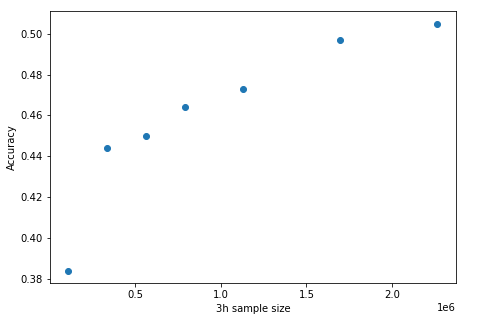
\includegraphics[width=0.8\textwidth]{accuracy_training_sample_size.png}
			\caption{The accuracy against 3h training sample size.}
			\label{fig:accuracy_training_sample_size}
		\end{figure}

	% subsection trainging_result_for_tri_higgs_events (end)	
	\subsection{Training curve}% (fold)
	\label{sub:training_curve}
		Figure \ref{fig:loss_and_accuracy_curve_no_btag_50_ep} and \ref{fig:loss_and_accuracy_curve_no_btag_100_ep} are the training curves for Case 9. After 50 epochs, the validation accuracy has not improved much.
		\begin{figure}[htpb]
			\centering
			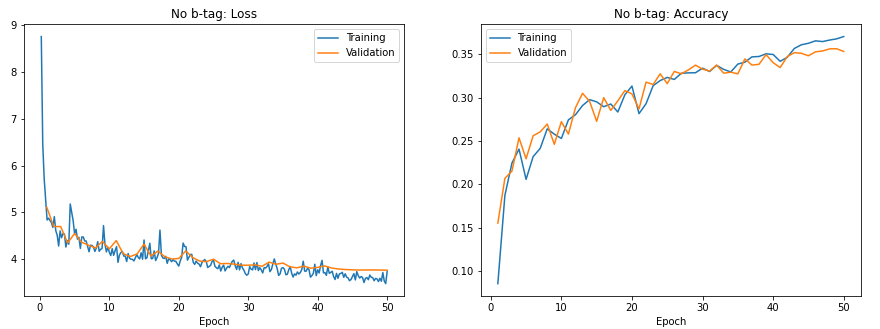
\includegraphics[width=0.9\textwidth]{loss_and_accuracy_curve_no_btag.png}
			\caption{The 50 epoch training curves for Case 9.}
			\label{fig:loss_and_accuracy_curve_no_btag_50_ep}
		\end{figure}

		\begin{figure}[htpb]
			\centering
			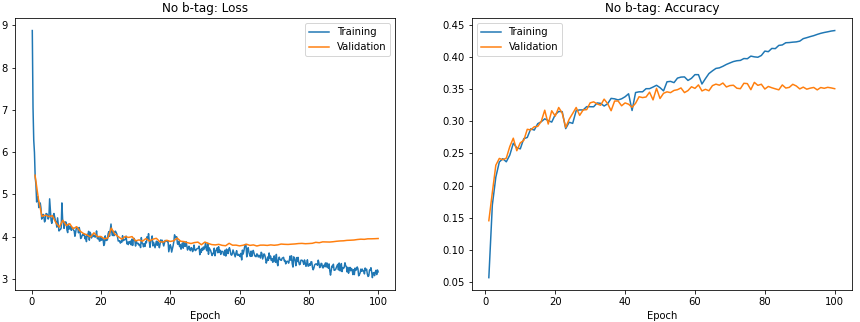
\includegraphics[width=0.9\textwidth]{loss_and_accuracy_curve_no_btag_100_ep.png}
			\caption{The 100 epoch training curves for Case 9.}
			\label{fig:loss_and_accuracy_curve_no_btag_100_ep}
		\end{figure}

		Figure \ref{fig:loss_and_accuracy_curve_6b_default} is the training curves for Case 10. 
		\begin{figure}[htpb]
			\centering
			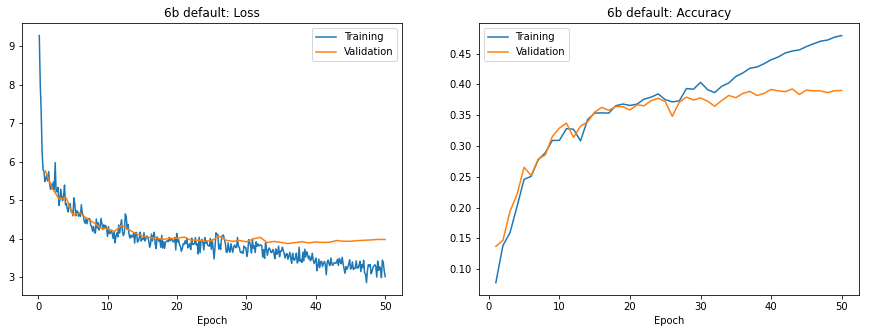
\includegraphics[width=0.9\textwidth]{loss_and_accuracy_curve_6b_default.png}
			\caption{The training curves for Case 10 (6b default).}
			\label{fig:loss_and_accuracy_curve_6b_default}
		\end{figure}
	% subsection training_curve (end)
	\subsection{Test on different dataset}% (fold)
	\label{sub:test_on_different_dataset}
		For example, use Case 5 samples for training and test on Case 5, 6, 7, and 8 samples. The results are presented in Table \ref{tab:SPANet_1M_0b_default_test_on_different_triHiggs_data}.
		\begin{table}[htpb]
			\centering
			\caption{0b SPANet test on different samples.}
			\label{tab:SPANet_1M_0b_default_test_on_different_triHiggs_data}
			\begin{tabular}{cc|cc}
				Training samples & Testing samples & Event efficiency & Higgs efficiency \\
				\hline 
				0b default      & 0b default     & 0.386        & 0.567    \\
				0b default      & 2b default     & 0.387        & 0.568    \\
				0b default      & 4b default     & 0.391        & 0.571    \\
				0b default      & 6b default     & 0.366        & 0.550    \\
			\end{tabular}
		\end{table}	

		Use Case 6 samples for training and test on Case 5, 6, 7, and 8 samples. The results are presented in Table \ref{tab:SPANet_1M_2b_default_test_on_different_triHiggs_data}.
		\begin{table}[htpb]
			\centering
			\caption{2b SPANet test on different samples.}
			\label{tab:SPANet_1M_2b_default_test_on_different_triHiggs_data}
			\begin{tabular}{cc|cc}
				Training samples & Testing samples & Event efficiency & Higgs efficiency \\
				\hline 
				2b default      & 0b default     & 0.383        & 0.562    \\
				2b default      & 2b default     & 0.383        & 0.562    \\
				2b default      & 4b default     & 0.388        & 0.565    \\
				2b default      & 6b default     & 0.363        & 0.548    \\
			\end{tabular}
		\end{table}	

		Use Case 7 samples for training and test on Case 5, 6, 7, and 8 samples. The results are presented in Table \ref{tab:SPANet_1M_4b_default_test_on_different_triHiggs_data}.
		\begin{table}[htpb]
			\centering
			\caption{4b SPANet test on different samples.}
			\label{tab:SPANet_1M_4b_default_test_on_different_triHiggs_data}
			\begin{tabular}{cc|cc}
				Training samples & Testing samples & Event efficiency & Higgs efficiency \\
				\hline 
				4b default      & 0b default     & 0.356        & 0.540    \\
				4b default      & 2b default     & 0.358        & 0.542    \\
				4b default      & 4b default     & 0.367        & 0.549    \\
				4b default      & 6b default     & 0.355        & 0.536    \\
			\end{tabular}
		\end{table}	

		Use Case 10 samples for training and test on Case 5, 6, 7, and 8 samples. The results are presented in Table \ref{tab:SPANet_10M_6b_default_test_on_different_triHiggs_data}.
		\begin{table}[htpb]
			\centering
			\caption{6b SPANet test on different samples.}
			\label{tab:SPANet_10M_6b_default_test_on_different_triHiggs_data}
			\begin{tabular}{cc|cc}
				Training samples & Testing samples & Event efficiency & Higgs efficiency \\
				\hline 
				6b default      & 0b default     & 0.230        & 0.412    \\
				6b default      & 2b default     & 0.234        & 0.417    \\
				6b default      & 4b default     & 0.290        & 0.476    \\
				6b default      & 6b default     & 0.385        & 0.559    \\
			\end{tabular}
		\end{table}	

		Use Case 12 samples for training and test on Case 6, 7, 10, and 12 samples. The results are presented in Table \ref{tab:SPANet_10M_0b_default_test_on_different_triHiggs_data}. 
		\begin{table}[htpb]
			\centering
			\caption{0b SPANet test on different samples.}
			\label{tab:SPANet_10M_0b_default_test_on_different_triHiggs_data}
			\begin{tabular}{cc|cc}
				Training samples & Testing samples & Event efficiency & Higgs efficiency \\
				\hline 
				0b default      & 0b default     & 0.473        & 0.632    \\
				0b default      & 2b default     & 0.475        & 0.634    \\
				0b default      & 4b default     & 0.479        & 0.636    \\
				0b default      & 6b default     & 0.457        & 0.623    \\
			\end{tabular}
		\end{table}	

		\begin{table}[htpb]
			\centering
			\caption{SPANet trained on 0b test on 6b.}
			\label{tab:SPANet_test_on_different_triHiggs_data}
			\begin{tabular}{c|c|cc}
				$N_\text{Jet}$ & Event Fraction & Event Efficiency & Higgs Efficiency \\
				\hline
				$=6$	  &   0.099             &    0.713              &    0.788             \\
				$=7$	  &   0.164             &    0.508              &    0.663             \\
				$\ge 8$	  &   0.269             &    0.331              &    0.538             \\
				Total	  &   0.533             &    0.457              &    0.623             \\
			\end{tabular}
		\end{table}

	% subsection test_on_different_dataset (end)	
% section spanet_for_tri_higgs_events_with_b_tag (end)		
\section{Hyperparameters}% (fold)
\label{sec:hyperparameters}
	Some hyperparameters of SPANet:
	\begin{itemize}
		\item Learning rate: 0.0004
		\item Central encoder count: 6
		\item Branch encoder count: 3
		\item Dropout percentage: 0.0
		\item L2 weight normalization: 0.0002
		\item L2 gradient clipping: 0.0
	\end{itemize}
	the above values are used in Sec.\ref{sec:spanet_for_tri_higgs_events_with_b_tag}.
	\subsection{Scan hyperparameters}% (fold)
	\label{sub:scan_hyperparameters}
		In below, use the 0b default samples (Sec.\ref{sub:trainging_result_for_tri_higgs_events}, Case 5) for hyperparameter scan.

		\paragraph{Learning rate} Range: $[0.0003,  0.0030]$. Step size: $0.0003$. Figure \ref{fig:SPANet_scan_lr} is the scanning results. The model cannot be trained when the learning rate is greater than 0.0006.
		\begin{figure}[htpb]
			\centering
			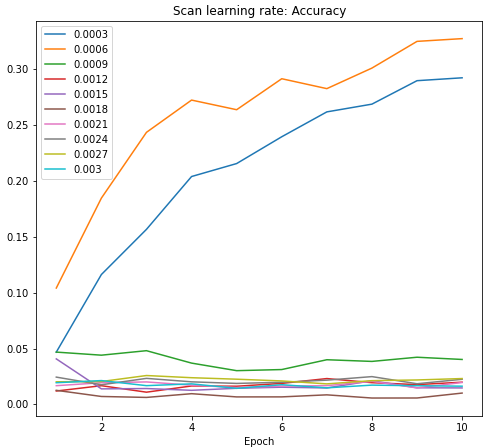
\includegraphics[width=0.6\textwidth]{accuracy_curve_hp_scan_lr.png}
			\caption{SPANet training results for different learning rates.}
			\label{fig:SPANet_scan_lr}
		\end{figure}

		\paragraph{Central encoder count} Range: $[2,6]$. Step size: $1$. Figure \ref{fig:SPANet_scan_n_cen} is the scanning results. When central encoder layers are equal to 2 or 4, the model will get the best performance at the first 10 epochs.
		\begin{figure}[htpb]
			\centering
			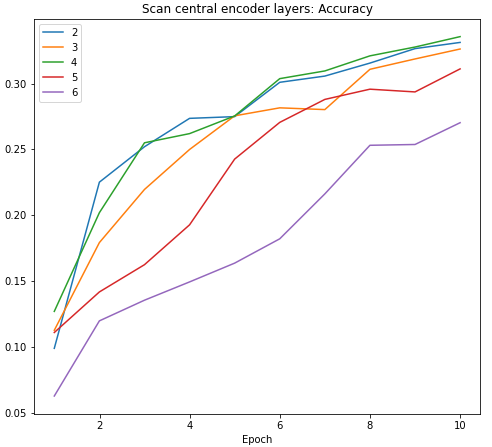
\includegraphics[width=0.6\textwidth]{accuracy_curve_hp_scan_n_cen.png}
			\caption{SPANet training results for different central encoder layers.}
			\label{fig:SPANet_scan_n_cen}
		\end{figure}

		\paragraph{Branch encoder count} Range: $[2,7]$. Step size: $1$. Figure \ref{fig:SPANet_scan_n_bren} is the scanning results. When branch encoder layers equal 2 or 4, the model will get the best performance at the first 10 epochs.
		\begin{figure}[htpb]
			\centering
			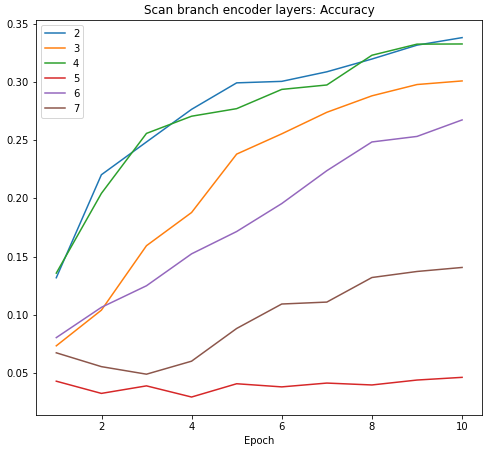
\includegraphics[width=0.6\textwidth]{accuracy_curve_hp_scan_n_bren.png}
			\caption{SPANet training results for different branch encoder layers.}
			\label{fig:SPANet_scan_n_bren}
		\end{figure}

	% subsection scan_hyperparameters (end)
	\subsection{Training results for different hyperparamers}% (fold)
	\label{sub:training_results_for_different_hyperparamers}
		In this section, use the 0b default samples (Sec.\ref{sub:trainging_result_for_tri_higgs_events}, Case 5) for training. Train 50 epochs. Table \ref{tab:SPANet_hp_50ep} is the training results for different hyperparameters.
		
		\begin{table}[htpb]
			\centering
			\caption{SPANet training results for different hyperparameters.}
			\label{tab:SPANet_hp_50ep}
			\begin{tabular}{cccc|cc}
			 & Central encoder & Branch encoder & learning rate & Event efficiency & Higgs efficiency \\
			 \hline
			 &    6             &     3           &  0.0004             &   0.386               &    0.567              \\
			 &    2             &     2           &  0.0006             &   0.395               &    0.571              \\
			 &    4             &     4           &  0.0006             &   0.362               &    0.547             \\
			 &    4             &     2           &  0.0006             &   0.386               &    0.567             
			\end{tabular}
		\end{table}
	% subsection training_results_for_different_hyperparamers (end)	
% section hyperparameters (end)		

\section{Signal and background}% (fold)
\label{sec:signal_and_background}
	To separate the signal and background events, defined the cuts as follows:
	\begin{itemize}
		\item Eta PT cut: In $\abs{\eta} < 2.5$ there are $\ge 6$ jets. The $p_\text{T}$ of jets are required over $25 \text{ GeV}$.
		\item bTag cut: $\ge 6$ b-jets.
		\item PT cut: Require 4 b-jets over $40 \text{ GeV}$.
		\item inv mass cut: The total invariant mass of 6 b-jets $\le 500 \text{ GeV}$.
	\end{itemize}

	The result is in Table \ref{tab:signal_background_analysis}.

	\begin{table}[htpb]
		\centering
		\caption{The cross sections for the signal and background processes at different cuts. $\mathcal{L} = 139 \text{ fb}^{-1}$ is provided.}
		\label{tab:signal_background_analysis}
		\begin{tabular}{l|ll|ll}
						 & \multicolumn{2}{|c|}{Cross section (pb)} &            &             \\
						 & Signal          & Background      & $S / B$        & $S / \sqrt{B}$ \\
			\hline 	
			No cut       & 0.0118         & 7.18e+02         & 1.64e-05 & 0.164       \\
			Eta PT cut   & 0.00619        & 29.6             & 0.000209 & 0.424       \\
			bTag cut     & 0.00199        & 0.711            & 0.0028   & 0.881       \\
			PT cut       & 0.00164        & 0.503            & 0.00326  & 0.86        \\
			inv mass cut & 0.0013         & 0.129            & 0.01     & 1.34       
		\end{tabular}
	\end{table}


	\subsection{With SPANet}% (fold)
	\label{sub:with_spanet}
		Define the cuts as follows:
		\begin{itemize}
			\item Eta PT cut: In $\abs{\eta} < 2.5$ there are $\ge 6$ jets. The $p_\text{T}$ of jets are required over $25 \text{ GeV}$.
			\item PT cut: Require 4 jets over $40 \text{ GeV}$.
			\item Higgs mass cut: Use the SPANet to pair the jets and calculate the invariant mass of Higgs. Require the mass difference of SM Higgs $\chi^2$ is smaller than $4000  \text{ GeV}^2$. The mass difference of SM Higgs $\chi^2$ is calculated as follows
			\[
				\chi^2 = [M(\text{b}_1\text{b}_2) - M_\text{H}]^2 + [M(\text{b}_3\text{b}_4) - M_\text{H}]^2 +[M(\text{b}_5\text{b}_6) - M_\text{H}]^2
			\] 
		\end{itemize}

		The result is in Table \ref{tab:signal_background_analysis_with_spanet}.

		\begin{table}[htpb]
			\centering
			\caption{The cross sections for the signal and background processes at different cuts.}
			\label{tab:signal_background_analysis_with_spanet}
			\begin{tabular}{l|ll|c|c|c|c}
							& \multicolumn{2}{|c|}{Cross section (fb)} &          & $\mathcal{L} = 139 \text{ fb}^{-1}$ & $\mathcal{L} = 300 \text{ fb}^{-1}$ & $\mathcal{L} = 3000 \text{ fb}^{-1}$ \\
						       & Signal           & Background          & $S / B$  & $S/\sqrt{B}$& $S/\sqrt{B}$& $S/\sqrt{B}$\\
				\hline		  
				No cut         & 11.8             & 7.18e+05            & 1.64e-05 & 0.164       & 0.241       & 0.761       \\
				Eta PT cut     & 6.19             & 2.96e+04            & 0.000209 & 0.424       & 0.623       & 1.97        \\
				PT cut         & 5.43             & 1.99e+04            & 0.000273 & 0.454       & 0.667       & 2.11        \\
				Higgs mass cut & 3.06             & 5.59e+03            & 0.000548 & 0.483       & 0.709       & 2.24       
			\end{tabular}
		\end{table}

		\subsubsection{Training SPANet}% (fold)
		\label{subs:training_spanet}
			The training samples are required to pass the ``Eta PT cut'' and ``PT cut'', $\ge 0$ b-tagged jets, b-tagging efficiency is the default.
			\begin{itemize}
				\item Training sample:
				\begin{itemize}
					\item Total sample size: 2,351,246
					\item 1h sample size: 782,136
					\item 2h sample size: 783,976
					\item 3h sample size: 477,070
					\item 5\% used on validation
				\end{itemize}
				\item Testing sample: 
				\begin{itemize}
					\item Total sample size: 261,717
					\item 1h sample size: 86,638
					\item 2h sample size: 87,394
					\item 3h sample size: 53,226
				\end{itemize}
			\end{itemize}
			The training results is presented in Table \ref{tab:SPANet_triHiggs_0btag_default_pt_cut}.
			\begin{table}[htpb]
				\centering
				\caption{SPA-NET training results on the ``PT cut'' samples.}
				\label{tab:SPANet_triHiggs_0btag_default_pt_cut}
				\begin{tabular}{c|c|cc}
					$N_\text{Jet}$ & Event Fraction & Event Efficiency & Higgs Efficiency \\
					\hline
					$=6$	  &   0.059             &    0.668              &    0.752             \\
					$=7$	  &   0.072             &    0.463              &    0.630             \\
					$\ge 8$	  &   0.072             &    0.297              &    0.509             \\
					Total	  &   0.203             &    0.464              &    0.623             \\
				\end{tabular}
			\end{table}
		% subsubsection training_spanet (end)	

	% subsection with_spanet (end)
% section signal_and_background (end)		
\section{Di-Higgs signal background analysis}% (fold)
\label{sec:di_higgs_signal_background_analysis}
	\subsection{Signal and background event}% (fold)
	\label{sub:signal_and_background_event}
		Signal: same as the di-Higgs events in Sec.\ref{sec:spanet_for_dihiggs_event}.

		Background: Generate background events in MadGraph by following commands:
		\begin{verbatim}
			define p = p b b~
			define j = j b b~
			generate p p > j j j j
		\end{verbatim}
	% subsection signal_and_background_event (end)
	

	\subsection{Cut}% (fold)
	\label{sub:cut}
		
		To separate the signal and background events, defined the cuts as follows:
		\begin{itemize}
			\item Eta PT cut: In $\abs{\eta} < 2.5$ there are $\ge 4$ jets. The $p_\text{T}$ of jets are required over $25 \text{ GeV}$.
			\item bTag cut: $\ge 2$ b-jets.
			% \item PT cut: Require 2 jets over $40 \text{ GeV}$.
			\item Higgs cut: Pair the jets and calculate the invariant mass of Higgs. Require the mass difference of SM Higgs $\chi^2$ is smaller than $1500 \text{ GeV}^2$. The mass difference of SM Higgs $\chi^2$ is calculated as follows
			\[
				\chi^2 = [M(\text{b}_1\text{b}_2) - M_\text{H}]^2 + [M(\text{b}_3\text{b}_4) - M_\text{H}]^2
			\] 
			The pairing methods are described below.
		\end{itemize}
		
		Pairing method 1: Minimize the mass difference of 2 Higgs candidates.

		Pairing method 2: Use the SPANet trained in Sec.\ref{sub:spanet_for_di_higgs_jet_pairing}.

		The result is in Table \ref{tab:diHiggs_signal_background_analysis}.
		\begin{table}[htpb]
			\centering
			\caption{The cross sections for the di-Higgs signal and background processes at different cuts. Higgs cut 1 is for method 1. Higgs cut 2 is for method 2.}
			\label{tab:diHiggs_signal_background_analysis}
			\begin{tabular}{l|ll|c|c|c|c}
						   & \multicolumn{2}{c|}{Cross section (fb)} &          & $\mathcal{L} = 139 \text{ fb}^{-1}$ & $\mathcal{L} = 300 \text{ fb}^{-1}$ & $\mathcal{L} = 3000 \text{ fb}^{-1}$ \\
						   & Signal           & Background           & $S / B$  & $S/\sqrt{B}$& $S/\sqrt{B}$& $S/\sqrt{B}$\\ \hline
				No cut     & 0.836            & 1.67e+07             & 5.02e-08 & 0.00242     & 0.00355     & 0.0112      \\
				Eta PT cut & 0.714            & 1.39e+07             & 5.15e-08 & 0.00226     & 0.00332     & 0.0105      \\
				bTag cut   & 0.575            & 8.78e+05             & 6.55e-07 & 0.00723     & 0.01060     & 0.0336      \\
				Higgs cut 1& 0.246            & 1.66e+05             & 1.48e-06 & 0.00711     & 0.01040     & 0.0330      \\
				Higgs cut 2& 0.302            & 1.09e+05             & 2.77e-06 & 0.01080     & 0.01580     & 0.0501     			
			\end{tabular}		
		\end{table}
	% subsection cut (end)

	\subsection{SPANet for di-Higgs jet pairing}% (fold)
	\label{sub:spanet_for_di_higgs_jet_pairing}
		The training samples are required to pass the ``Eta PT cut'', $\ge 2$ b-tagged jets. The b-tagging efficiency is the default.
		\begin{itemize}
			\item Training sample:
			\begin{itemize}
				\item Total sample size: 617,340
				\item 1h sample size: 266,790
				\item 2h sample size: 315,219
				\item 5\% used on validation
			\end{itemize}
			\item Testing sample: 
			\begin{itemize}
				\item Total sample size: 68,626
				\item 1h sample size: 29,506
				\item 2h sample size: 35,265
			\end{itemize}
		\end{itemize}
		The training results is presented in Table \ref{tab:SPANet_diHiggs_2btag_default_pt_cut}.
		\begin{table}[htpb]
			\centering
			\caption{SPA-NET training results on the di-Higgs samples with ``Eta PT cut'' and ``bTag cut''.}
			\label{tab:SPANet_diHiggs_2btag_default_pt_cut}
			\begin{tabular}{c|c|cc}
				$N_\text{Jet}$ & Event Fraction & Event Efficiency & Higgs Efficiency \\
				\hline
				$=4$	  &   0.129             &    1.000              &    1.000             \\
				$=5$	  &   0.178             &    0.968              &    0.984             \\
				$\ge 6$	  &   0.207             &    0.895              &    0.946             \\
				Total	  &   0.514             &    0.947              &    0.973             \\
			\end{tabular}
		\end{table}

	% subsection spanet_for_di_higgs_jet_pairing (end)
	
	\subsection{ATLAS}% (fold)
	\label{sub:atlas}
		The selection steps:
		\begin{itemize}
			\item Four tag: The event contains at least 4 b-tagged anti-kt small-$R$ ($R = 0.4$) jets with $p_\text{T} > \text{40 GeV}$ and $\abs{\eta} < 2.5$. The four jets with the highest b-tagging score are paired to construct two Higgs boson candidates.
			\item The four jets with the highest $p_\text{T}$ are paired to construct two Higgs boson candidates in my samples.
			\item Delta R: Pairing jets to Higgs boson candidate need to satisfy the following requirements:
			\[
				\left.
				\begin{array}{c}
					\dfrac{\text{360 GeV}}{m_\text{4j}} - 0.5 < \Delta R_{jj,\text{lead}} < \dfrac{\text{653 GeV}}{m_{\text{4j}}} + 0.475 \\
					\dfrac{\text{235 GeV}}{m_\text{4j}}  < \Delta R_{jj,\text{subl}} < \dfrac{\text{875 GeV}}{m_{\text{4j}}} + 0.35 
				\end{array} 
				\right\} \text{ if } m_{\text{4j}} <  \text{1250 GeV}
			\] 
			\[
				\left.
				\begin{array}{c}
					0 < \Delta R_{jj,\text{lead}} < 1 \\
					0 < \Delta R_{jj,\text{subl}} < 1 
				\end{array} 
				\right\} \text{ if } m_{\text{4j}} >  \text{1250 GeV}
			\] 
			\item If there are more than 2 pairings satisfy the Delta R requirement. Calculate $D_{HH}$
			\[
				D_{HH} = \frac{\abs{m_{\text{2j}}^{\text{lead}} - \frac{120}{110} m_{\text{2j}}^{\text{subl}}}}{\sqrt{1 + \left( \frac{120}{110} \right)^2}}
			\] 
			the pairing with the smallest value of $D_{HH}$ is chosen.
			\item Higgs PT: 
			\begin{align*}
				p_{\text{T}}^{\text{lead}} &> m_{\text{4j}} \times 0.5 - \text{103 GeV} \\
				p_{\text{T}}^{\text{subl}} &> m_{\text{4j}} \times 0.33 - \text{73 GeV} \\
			\end{align*}
			\item Higgs Eta: 
			\[
				\abs{\Delta\eta_{HH}} < 1.5
			\] 
			\item Signal region:
			\[
				X_{HH} = \sqrt{\left( \frac{m_{\text{2j}}^{\text{lead}} - \text{120 GeV}}{0.1 m_{\text{2j}}^{\text{lead}}} \right)^2 + \left(\frac{m_{\text{2j}}^{\text{subl}} - \text{110 GeV}}{0.1 m_{\text{2j}}^{\text{subl}}} \right)^2} < 1.6
			\]
			\item Top veto: Every possible pair of jets with $p_\text{T} > \text{40 GeV}$ and $\abs{\eta} < 2.5$, including those that were not selected for the $H$ candidates, to form ``$W$ candidates''. ``Top quark candidates'' are built by pairing $W$ candidates with each remaining jet that was selected for $H$ candidates
			\[
				X_{Wt} = \sqrt{\left( \frac{m_{W} - \text{80 GeV}}{0.1 m_{W}} \right)^2 + \left(\frac{m_{t} - \text{173 GeV}}{0.1 m_{t}} \right)^2} 
			\] 
			Events with the smallest $X_{Wt} < 1.5$ are vetoed.

		\end{itemize}

		Test the above selection steps on the $\text{13 TeV}$ samples with $m_{H_2} = \text{1000 GeV}$ and compare the results with ATLAS paper (Figure \ref{fig:ATLAS_signal_selection}). The result is in Table \ref{tab:signal_selection_efficiency_1000GeV}. The biggest difference is at Delta R cut. 
		\begin{figure}[htpb]
			\centering
			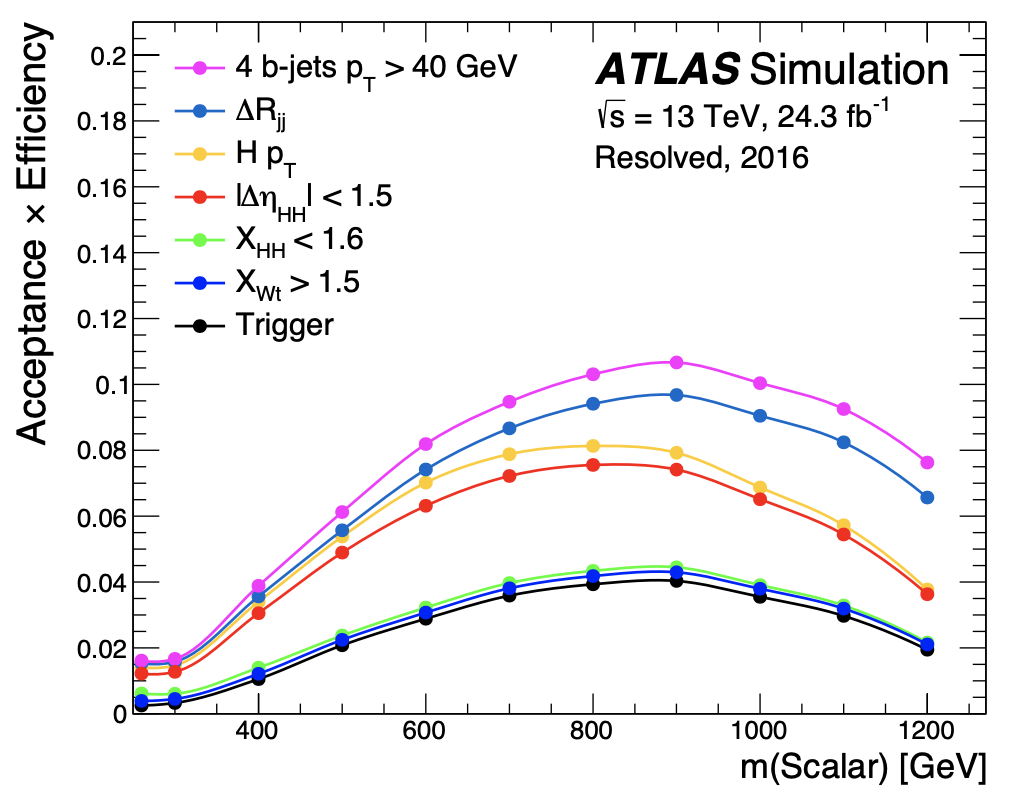
\includegraphics[width=0.8\textwidth]{ATLAS_signal_selection.png}
			\caption{The selection acceptance times efficiency at each stage for the scalar.}
			\label{fig:ATLAS_signal_selection}
		\end{figure}
		\begin{table}[htpb]
			\centering
			\caption{The selection passing rate and efficiency at each stage. The resonant mass is $\text{1000 GeV}$.}
			\label{tab:signal_selection_efficiency_1000GeV}
			\begin{tabular}{l|cc|cc}
							  & \multicolumn{2}{|c|}{ATLAS 1000 GeV} & \multicolumn{2}{|c}{My sample 1000 GeV} \\
				Cut           & pass rate       & efficiency       & pass rate         & efficiency         \\ \hline
				Four tag      & 0.1000 & 0.1000 & 0.1386 & 0.1386 \\
				Delta R       & 0.0900 & 0.9003 & 0.1089 & 0.7856 \\
				Higgs PT      & 0.0683 & 0.7584 & 0.0871 & 0.7996 \\
				Higgs Eta     & 0.0647 & 0.9469 & 0.0803 & 0.9225 \\
				Signal region & 0.0390 & 0.6028 & 0.0422 & 0.5251 \\
				Top veto      & 0.0375 & 0.9612 & 0.0418 & 0.9912
			\end{tabular}
		\end{table}

		\begin{table}[htpb]
			\centering
			\caption{The selection passing rate and efficiency at each stage. The resonant mass is $\text{600 GeV}$.}
			\label{tab:signal_selection_efficiency_600GeV}
			\begin{tabular}{l|cc|cc}
							  & \multicolumn{2}{c}{ATLAS 600 GeV} & \multicolumn{2}{|c}{My sample 600 GeV} \\
				Cut           & pass rate   & efficiency  & pass rate     & efficiency    \\ \hline
				Four tag      & 0.0821      & 0.0821      & 0.1120        & 0.1120        \\
				Delta R       & 0.0739      & 0.9004      & 0.0856        & 0.7645        \\
				Higgs PT      & 0.0703      & 0.9508      & 0.0820        & 0.9571        \\
				Higgs Eta     & 0.0630      & 0.8966      & 0.0734        & 0.8951        \\
				Signal region & 0.0324      & 0.5144      & 0.0287        & 0.3915        \\
				Top veto      & 0.0306      & 0.9439      & 0.0284        & 0.9903       	
			\end{tabular}
		\end{table}


		\subsubsection{Delta R cut}% (fold)
		\label{subs:delta_r_cut}
			Change the b-tagging efficiency in Delphes such that the ``Four tag'' efficiency is the same as the ATLAS results. The b-tagging efficiency after the change is
			\begin{equation}\label{eq:b_tagging_efficiency_2}
				\text{eff.} = 0.78 \tanh(0.0025p_\text{T}) \frac{25.0}{1+0.063p_\text{T}}		
			\end{equation}
			Generate events and apply the selection again. The results are in Table \ref{tab:signal_selection_efficiency_1000GeV_change_btag}.
			\begin{table}[htpb]
				\centering
				\caption{The selection passing rate and efficiency at each stage. The b-tagging efficiency is (\ref{eq:b_tagging_efficiency_2}). The resonant mass is $\text{1000 GeV}$.}
				\label{tab:signal_selection_efficiency_1000GeV_change_btag}
				\begin{tabular}{l|cc|cc}
								  & \multicolumn{2}{|c|}{ATLAS 1000 GeV} & \multicolumn{2}{|c}{My sample 1000 GeV} \\
					Cut           & pass rate       & efficiency       & pass rate         & efficiency         \\ \hline
					Four tag      & 0.1000 & 0.1000 & 0.1006 & 0.1006 \\
					Delta R       & 0.0900 & 0.9003 & 0.0781 & 0.7758 \\
					Higgs PT      & 0.0683 & 0.7584 & 0.0627 & 0.8036 \\
					Higgs Eta     & 0.0647 & 0.9469 & 0.0575 & 0.9173 \\
					Signal region & 0.0390 & 0.6028 & 0.0297 & 0.5163 \\
					Top veto      & 0.0375 & 0.9612 & 0.0294 & 0.9906      
				\end{tabular}
			\end{table}
			
			Define the correct jet assignments by matching them to the simulated truth quarks within an angular distance of $\Delta R = \sqrt{\Delta\eta^2 + \Delta\phi^2}<0.4$.

		The four b-jets with the highest $p_\text{T}$ are paired to construct two Higgs boson candidates in my samples. When I checked the truth matching, I found the four b-jets may not all decay from Higgs. The event with a b-jet does not decay from Higgs is hard to pass the ``Delta R cut''. The number is in Table \ref{tab:signal_selection_compared_with_truth_matching_1000GeV}. 
			\begin{table}[htpb]
				\centering
				\caption{Unmatched are the events that cannot define the correct jet assignments. Use the correct jet assignments to determine if four b-jets are all from Higgs. The total number of events is 100k. The resonant mass is $\text{1000 GeV}$.}
				\label{tab:signal_selection_compared_with_truth_matching_1000GeV}
				\begin{tabular}{l|c|ccc}
							 & Total & All from Higgs & Not all from Higgs & Unmatched\\ \hline
					Four tag & 13863 & 9348    & 2536  & 1979   \\
					Delta R  & 10891 & 8961    & 857   & 1073    
				\end{tabular}
			\end{table}

		% subsubsection delta_r_cut (end)
		\subsubsection{Change b-tag efficiency}% (fold)
		\label{subs:change_b_tag_efficiency}
			Change the b-tagging part in the Delphes card such that same as the MV2c10 b-tagger at 70\% WP. 

			The b-jet efficiency is set to 0.70. The c-jet missing rate is set to 0.083. The light jet missing rate is set to 0.0026.

			Regenerate the events and apply the cut. The result is in Table \ref{tab:signal_selection_efficiency_1000GeV_MV2c10}. The Delta R cut efficiency is 0.86, has a big difference compared to the before result of 0.78.

			\begin{table}[htpb]
				\centering
				\caption{The selection passing rate and efficiency at each stage. The b-tagging part is the same as the MV2c10 70\% WP. The resonant mass is $\text{1000 GeV}$.}
				\label{tab:signal_selection_efficiency_1000GeV_MV2c10}
				\begin{tabular}{l|cc|cc}
								  & \multicolumn{2}{|c|}{ATLAS 1000 GeV} & \multicolumn{2}{|c}{My sample 1000 GeV} \\
					Cut           & pass rate       & efficiency       & pass rate         & efficiency         \\ \hline
					Four tag      & 0.1000 & 0.1000 & 0.1257 & 0.1257 \\
					Delta R       & 0.0900 & 0.9003 & 0.1087 & 0.8643 \\
					Higgs PT      & 0.0683 & 0.7584 & 0.0896 & 0.8247 \\
					Higgs Eta     & 0.0647 & 0.9469 & 0.0826 & 0.9216 \\
					Signal region & 0.0390 & 0.6028 & 0.0445 & 0.5391 \\
					Top veto      & 0.0375 & 0.9612 & 0.0441 & 0.9899
				\end{tabular}
			\end{table}

			\begin{table}[htpb]
				\centering
				\caption{Unmatched are the events that cannot define the correct jet assignments. Use the correct jet assignments to determine if four b-jets are all from Higgs. The total number of events is 100k. The b-tagging part is the same as the MV2c10 70\% WP. The resonant mass is $\text{1000 GeV}$.}
				\label{tab:signal_selection_compared_with_truth_matching_1000GeV_MV2c10}
				\begin{tabular}{l|c|ccc}
							 & Total & All from Higgs & Not all from Higgs & Unmatched \\ \hline
					Four tag & 12573 & 10041    & 1181  & 1351   \\
					Delta R  & 10868 & 9635    & 337   & 856    
				\end{tabular}
			\end{table}

		% subsubsection change_b_tag_efficiency (end)		
		\subsubsection{Training SPANet for jet pairing}% (fold)
		\label{subs:training_spanet_for_jet_pairing}
			The training samples are required to pass the ``Four tag cut'', i.e., there are at least four b-tagged jets with $p_{\text{T}} > \text{40 GeV}$ and $\abs{\eta} < 2.5$. The b-tagging efficiency is the same as the MV2c10 b-tagger at 70\% WP.
			\begin{itemize}
				\item Training sample:
				\begin{itemize}
					\item Total sample size: 109,252
					\item 1h sample size: 11,746
					\item 2h sample size: 97,053
					\item 5\% used on validation
				\end{itemize}
				\item Testing sample: 
				\begin{itemize}
					\item Total sample size: 12,140
					\item 1h sample size: 1,199
					\item 2h sample size: 10,883
				\end{itemize}
			\end{itemize}
			The training results is presented in Table \ref{tab:SPANet_diHiggs_4btag_MV2c10_pt40}.
			\begin{table}[htpb]
				\centering
				\caption{SPA-NET training results on the di-Higgs samples with ``Four tag cut''.}
				\label{tab:SPANet_diHiggs_4btag_MV2c10_pt40}
				\begin{tabular}{c|c|cc}
					$N_\text{Jet}$ & Event Fraction & Event Efficiency & Higgs Efficiency \\
					\hline
					$=4$	  &   0.307             &    1.000              &    1.000             \\
					$=5$	  &   0.365             &    0.968              &    0.984             \\
					$\ge 6$	  &   0.264             &    0.906              &    0.951             \\
					Total	  &   0.896             &    0.961              &    0.980             \\
				\end{tabular}
			\end{table}
	
		% subsubsection training_spanet_for_jet_pairing (end)
		\subsubsection{Use SPANet for event selection}% (fold)
		\label{subs:use_spanet_for_event_selection}
			The ``$\Delta R + \text{min-}D_{HH}$'' pairing is replaced by SPANet pairing. Other cuts are will remain unchanged. The result is in Table \ref{tab:signal_selection_efficiency_1000GeV_MV2c10_SPANet}.
			\begin{table}[htpb]
				\centering
				\caption{The selection passing rate and efficiency at each stage for ``$\Delta R + \text{min-}D_{HH}$'' and SPA-NET pairing. The resonant mass is $\text{1000 GeV}$.}
				\label{tab:signal_selection_efficiency_1000GeV_MV2c10_SPANet}
				\begin{tabular}{l|cc|cc|cc}
						& \multicolumn{4}{c|}{$\Delta R + \text{min-}D_{HH}$}                               & \multicolumn{2}{c}{SPA-NET}   \\
								  & \multicolumn{2}{c|}{ATLAS} & \multicolumn{2}{c|}{My sample}             & \multicolumn{2}{c}{My sample} \\
					Cut           & pass rate   & efficiency  & pass rate & \multicolumn{1}{c|}{efficiency} & pass rate     & efficiency    \\ \hline
					Four tag      & 0.1000      & 0.1000      & 0.1257    & 0.1257                          & 0.1257        & 0.1257        \\
					Delta R       & 0.0900      & 0.9003      & 0.1087    & 0.8643                          & N.A.          & N.A.          \\
					Higgs PT      & 0.0683      & 0.7584      & 0.0896    & 0.8247                          & 0.0976        & 0.7759        \\
					Higgs Eta     & 0.0647      & 0.9469      & 0.0826    & 0.9216                          & 0.0898        & 0.9202        \\
					Signal region & 0.0390      & 0.6028      & 0.0445    & 0.5391                          & 0.0468        & 0.5213        \\
					Top veto      & 0.0375      & 0.9612      & 0.0441    & 0.9899                          & 0.0463        & 0.9897   
				\end{tabular}
			\end{table}

			To separate the signal and background, apply the same selection steps to both samples. The background process is pp->4b. The ``$\Delta R + \text{min-}D_{HH}$'' result is in Table \ref{tab:diHiggs_signal_background_analysis_ATLAS_minDHH}. The SPANet result is in Table \ref{tab:diHiggs_signal_background_analysis_ATLAS_SPANet}. After the ``Signal region cut'', the SPANet pairing method has an improvement on $S/\sqrt{B}$.
			\begin{table}[htpb]
				\centering
				\caption{The cross sections for the di-Higgs signal and background processes at different cuts. The pairing method is ``$\Delta R + \text{min-}D_{HH}$''.}
				\label{tab:diHiggs_signal_background_analysis_ATLAS_minDHH}
				\begin{tabular}{l|cc|c|c|c|c}
								  & \multicolumn{2}{c|}{Cross section (fb)} &          & $\mathcal{L} = 139 \text{ fb}^{-1}$ & $\mathcal{L} = 300 \text{ fb}^{-1}$ & $\mathcal{L} = 3000 \text{ fb}^{-1}$ \\
								  & Signal           & Background           & $S / B$  & $S/\sqrt{B}$                        & $S/\sqrt{B}$                        & $S/\sqrt{B}$                         \\ \hline
					No cut        & 0.644            & 6.29e+05             & 1.02e-06 & 0.00958                             & 0.0141                              & 0.0445                               \\
					Four tag      & 0.081            & 5.9e+03              & 1.37e-05 & 0.0124                              & 0.0183                              & 0.0577                               \\
					Delta R       & 0.070            & 2.94e+03             & 2.38e-05 & 0.0152                              & 0.0224                              & 0.0708                               \\
					Higgs PT & 0.058            & 2.46e+03             & 2.34e-05 & 0.0137                              & 0.0201                              & 0.0637                               \\
					Higgs Eta & 0.053            & 1.78e+03             & 2.99e-05 & 0.0149                              & 0.0219                              & 0.0691                               \\
					Signal region  & 0.029            & 3.58e+02             & 8.01e-05 & 0.0179                              & 0.0262                              & 0.0830                               \\
					Top veto      & 0.028            & 3.58e+02             & 7.93e-05 & 0.0177                              & 0.0260                              & 0.0822                              
				\end{tabular}
			\end{table}

			\begin{table}[htpb]
				\centering
				\caption{The cross sections for the di-Higgs signal and background processes at different cuts. The pairing method is SPA-NET.}
				\label{tab:diHiggs_signal_background_analysis_ATLAS_SPANet}
				\begin{tabular}{l|cc|c|c|c|c}
								  & \multicolumn{2}{c|}{Cross section (fb)} &          & $\mathcal{L} = 139 \text{ fb}^{-1}$ & $\mathcal{L} = 300 \text{ fb}^{-1}$ & $\mathcal{L} = 3000 \text{ fb}^{-1}$ \\
								  & Signal           & Background           & $S / B$  & $S/\sqrt{B}$                        & $S/\sqrt{B}$                        & $S/\sqrt{B}$                         \\ \hline
					No cut        & 0.644            & 6.29e+05             & 1.02e-06 & 0.00958                             & 0.0141                              & 0.0445                               \\
					Four tag      & 0.081            & 6.06e+03             & 1.34e-05 & 0.0123                              & 0.018                               & 0.0570                                \\
					Higgs PT & 0.063            & 4.07e+03             & 1.54e-05 & 0.0116                              & 0.0171                              & 0.0540                               \\
					Higgs Eta & 0.058            & 3e+03                & 1.93e-05 & 0.0124                              & 0.0183                              & 0.0578                               \\
					Signal region  & 0.030            & 52.2                 & 0.000578 & 0.0492                              & 0.0723                              & 0.2290                               \\
					Top veto      & 0.030            & 52.2                 & 0.000572 & 0.0487                              & 0.0716                              & 0.2260                              
				\end{tabular}	
			\end{table}

		% subsubsection use_spanet_for_event_selection (end)		
	% subsection atlas (end)	
		



% section di_higgs_signal_background_analysis (end)			
\end{document} 
